\chapter{Results}
\label{ch:results}

This chapter presents the experimental results for the two benchmark models introduced in \cref{sec:ocp_spacecraft,sec:ocp_arm7}. 
The results are organized by physical model to analyze individually the algorithms performances on each model. 
Within each model, the algorithms are compared using the evaluation metrics defined in \cref{sec:setup_metrics}.

\section{Evaluation Protocol}
\label{sec:results_protocol}

\todoX{State the number of independent runs, random seeds, test cases, and the workstation used for each result reported in this chapter.}
\todoX{State how failed runs, timeouts, infeasible solutions, and missing measurements are handled in the tables and plots.}
\todoX{Confirm the statistical summaries reported throughout this chapter: success rate, computation time, objective cost, constraint violation, and solution diversity.}

The algorithms' performances over the three evaluation runs---the spacecraft slew test cases, 1000-\ac{LUT} robotic manipulator 
test cases, and 100-\ac{LUT} global landscape robotic manipulator test cases---are evaluated
according to reliability, computation time, and solution quality. Relevant statistical summaries including 
success rate, computation time, objective cost, and solution diversity are reported.
At the end of each evaluation set's reported data, a discussion highlighting the key findings
is performed.

\section{Spacecraft Attitude Slew Results}
\label{sec:results_spacecraft}

\subsection{Spacecraft Results Discussion}
\label{sec:results_spacecraft_discussion}

\todoX{Summarize the main spacecraft findings and connect them to the algorithm mechanisms discussed in \cref{sec:algorithm_frameworks}.}
\todoX{Identify which methods are most reliable, fastest, and most effective at finding low-cost or diverse solutions.}

\section{Robotic Manipulator Ball-Catching Results}
\label{sec:results_manipulator}

The results of the robotic manipulator ball-catching experiments consist of two 
evaluation sets: the 1,000-\ac{LUT} test cases and the 100-\ac{LUT} global landscape 
test cases. 
The 1000-\ac{LUT} test cases are used to evaluate the algorithms' 
performance on a large set ball velocities. 
This set's primary purpose is to compare against the results obtained during 
Lampariello et al.'s 2011 study \cite{Lampariello2011}.
In this study, a Monte Carlo-based global search was performed to establish 
reference solutions for the test cases.
As each algorithm's individual test case terminates upon finding a first solution, this
set primarily evaluates the algorithms' ability to quickly find feasible solutions and 
the quality of that initial solution.
In contrast, the 100-\ac{LUT} evaluation set focuses on a global landscape study of the
solution space. 
This evaluation set is designed to assess the algorithms' ability to explore the solution 
space comprehensively and identify high-quality solutions beyond the initial feasible ones.

\subsection{1000\ac{LUT}-Runs Evaluation Set}

\begin{table}[ht]
\centering
\caption{Per-test-case best-cost groups, treating costs within 0.5\% of the minimum as equivalent.}
\label{tab:best-cost-winner-groups}
\begin{tabular}{lr}
\hline
Best-cost winner group & Number of rows \\
\hline
MC & 1 \\
P-HO & 23 \\
RRT*-GBO & 8 \\
Local GBO & 0 \\
MC + P-HO & 6 \\
MC + RRT*-GBO & 6 \\
MC + Local GBO & 4 \\
P-HO + RRT*-GBO & 2 \\
P-HO + Local GBO & 4 \\
RRT*-GBO + Local GBO & 1 \\
MC + P-HO + RRT*-GBO & 12 \\
MC + P-HO + Local GBO & 56 \\
MC + RRT*-GBO + Local GBO & 12 \\
P-HO + RRT*-GBO + Local GBO & 17 \\
MC + P-HO + RRT*-GBO + Local GBO & 848 \\
\hline
Total & 1000 \\
\hline
\end{tabular}
\end{table}

\begin{table}[ht]
\centering
\caption{Per-test-case wall-clock runtime summary in seconds.}
\label{tab:runtime-summary}
\begin{tabular}{lrrrr}
\hline
Algorithm & $n$ & Median (s) & $Q_1$--$Q_3$ (s) & $P_{10}$--$P_{90}$ (s) \\
\hline
MC & 1000 & 360.9 & 295.6--624.9 & 170.7--834.1 \\
P-HO & 1000 & 342.7 & 231.3--434.3 & 192.2--536.3 \\
RRT*-GBO & 1000 & 59.5 & 47.3--113.2 & 42.9--1019.5 \\
Local GBO & 1000 & 53.0 & 42.3--132.9 & 35.3--190.4 \\
\hline
\end{tabular}
\end{table}

\begin{table}[ht]
\centering
\caption{Per-test-case costs compared with the \ac{LUT} reference; differences within 0.5\% are equivalent.}
\label{tab:csv-cost-comparison}
\begin{tabular}{lrrrrr}
\hline
Algorithm & Better & Equivalent & Worse & No feasible cost & Total rows \\
\hline
MC & 7 & 943 & 43 & 7 & 1000 \\
P-HO & 13 & 956 & 27 & 4 & 1000 \\
RRT*-GBO & 9 & 899 & 31 & 61 & 1000 \\
Local GBO & 5 & 944 & 42 & 9 & 1000 \\
\hline
\end{tabular}
\end{table}


\begin{figure}[htbp]
\centering
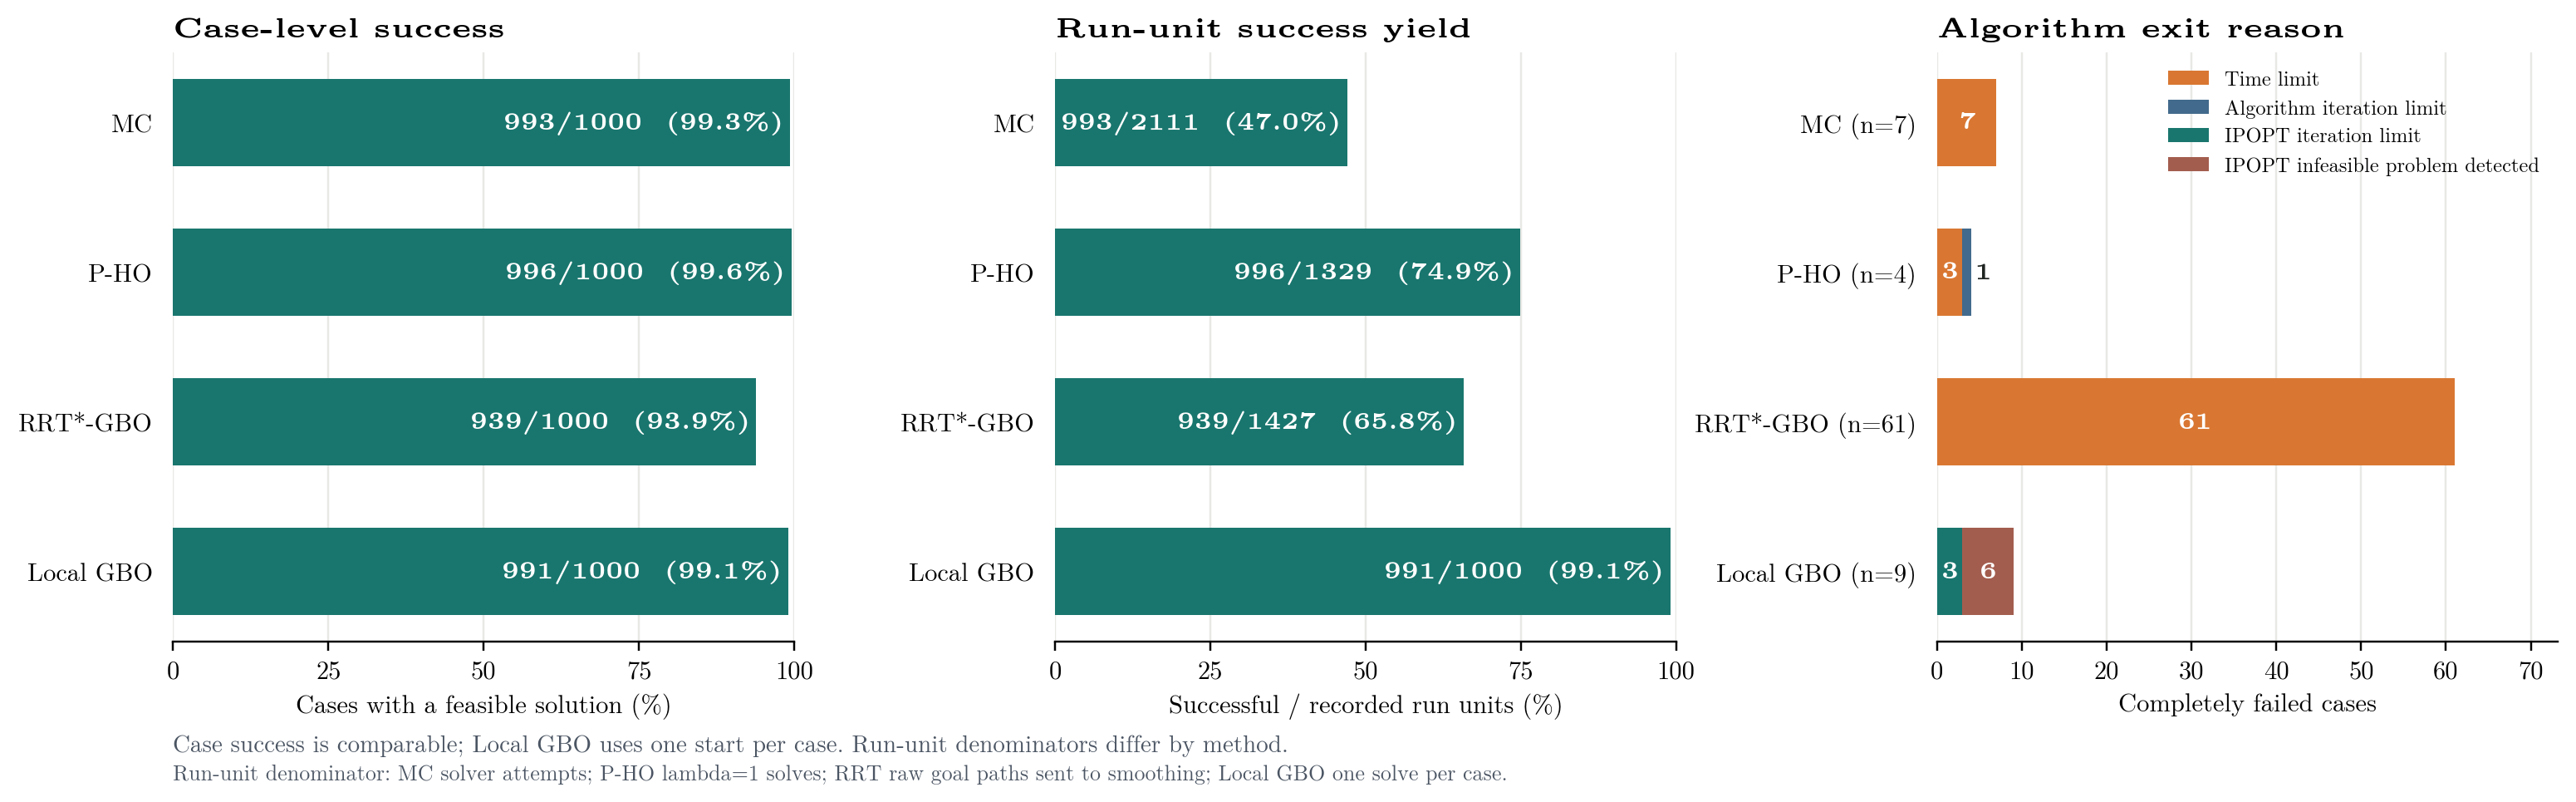
\includegraphics[width=\textwidth]{images/1000LUTRuns/reliability.png}
\caption{Reliability of the four algorithms over the 1,000 manipulator test cases. Case-level success, run-unit success yield, and completely failed cases are shown together with the corresponding termination reasons.}
\label{fig:manipulator-reliability}
\end{figure}

\begin{figure}[htbp]
\centering
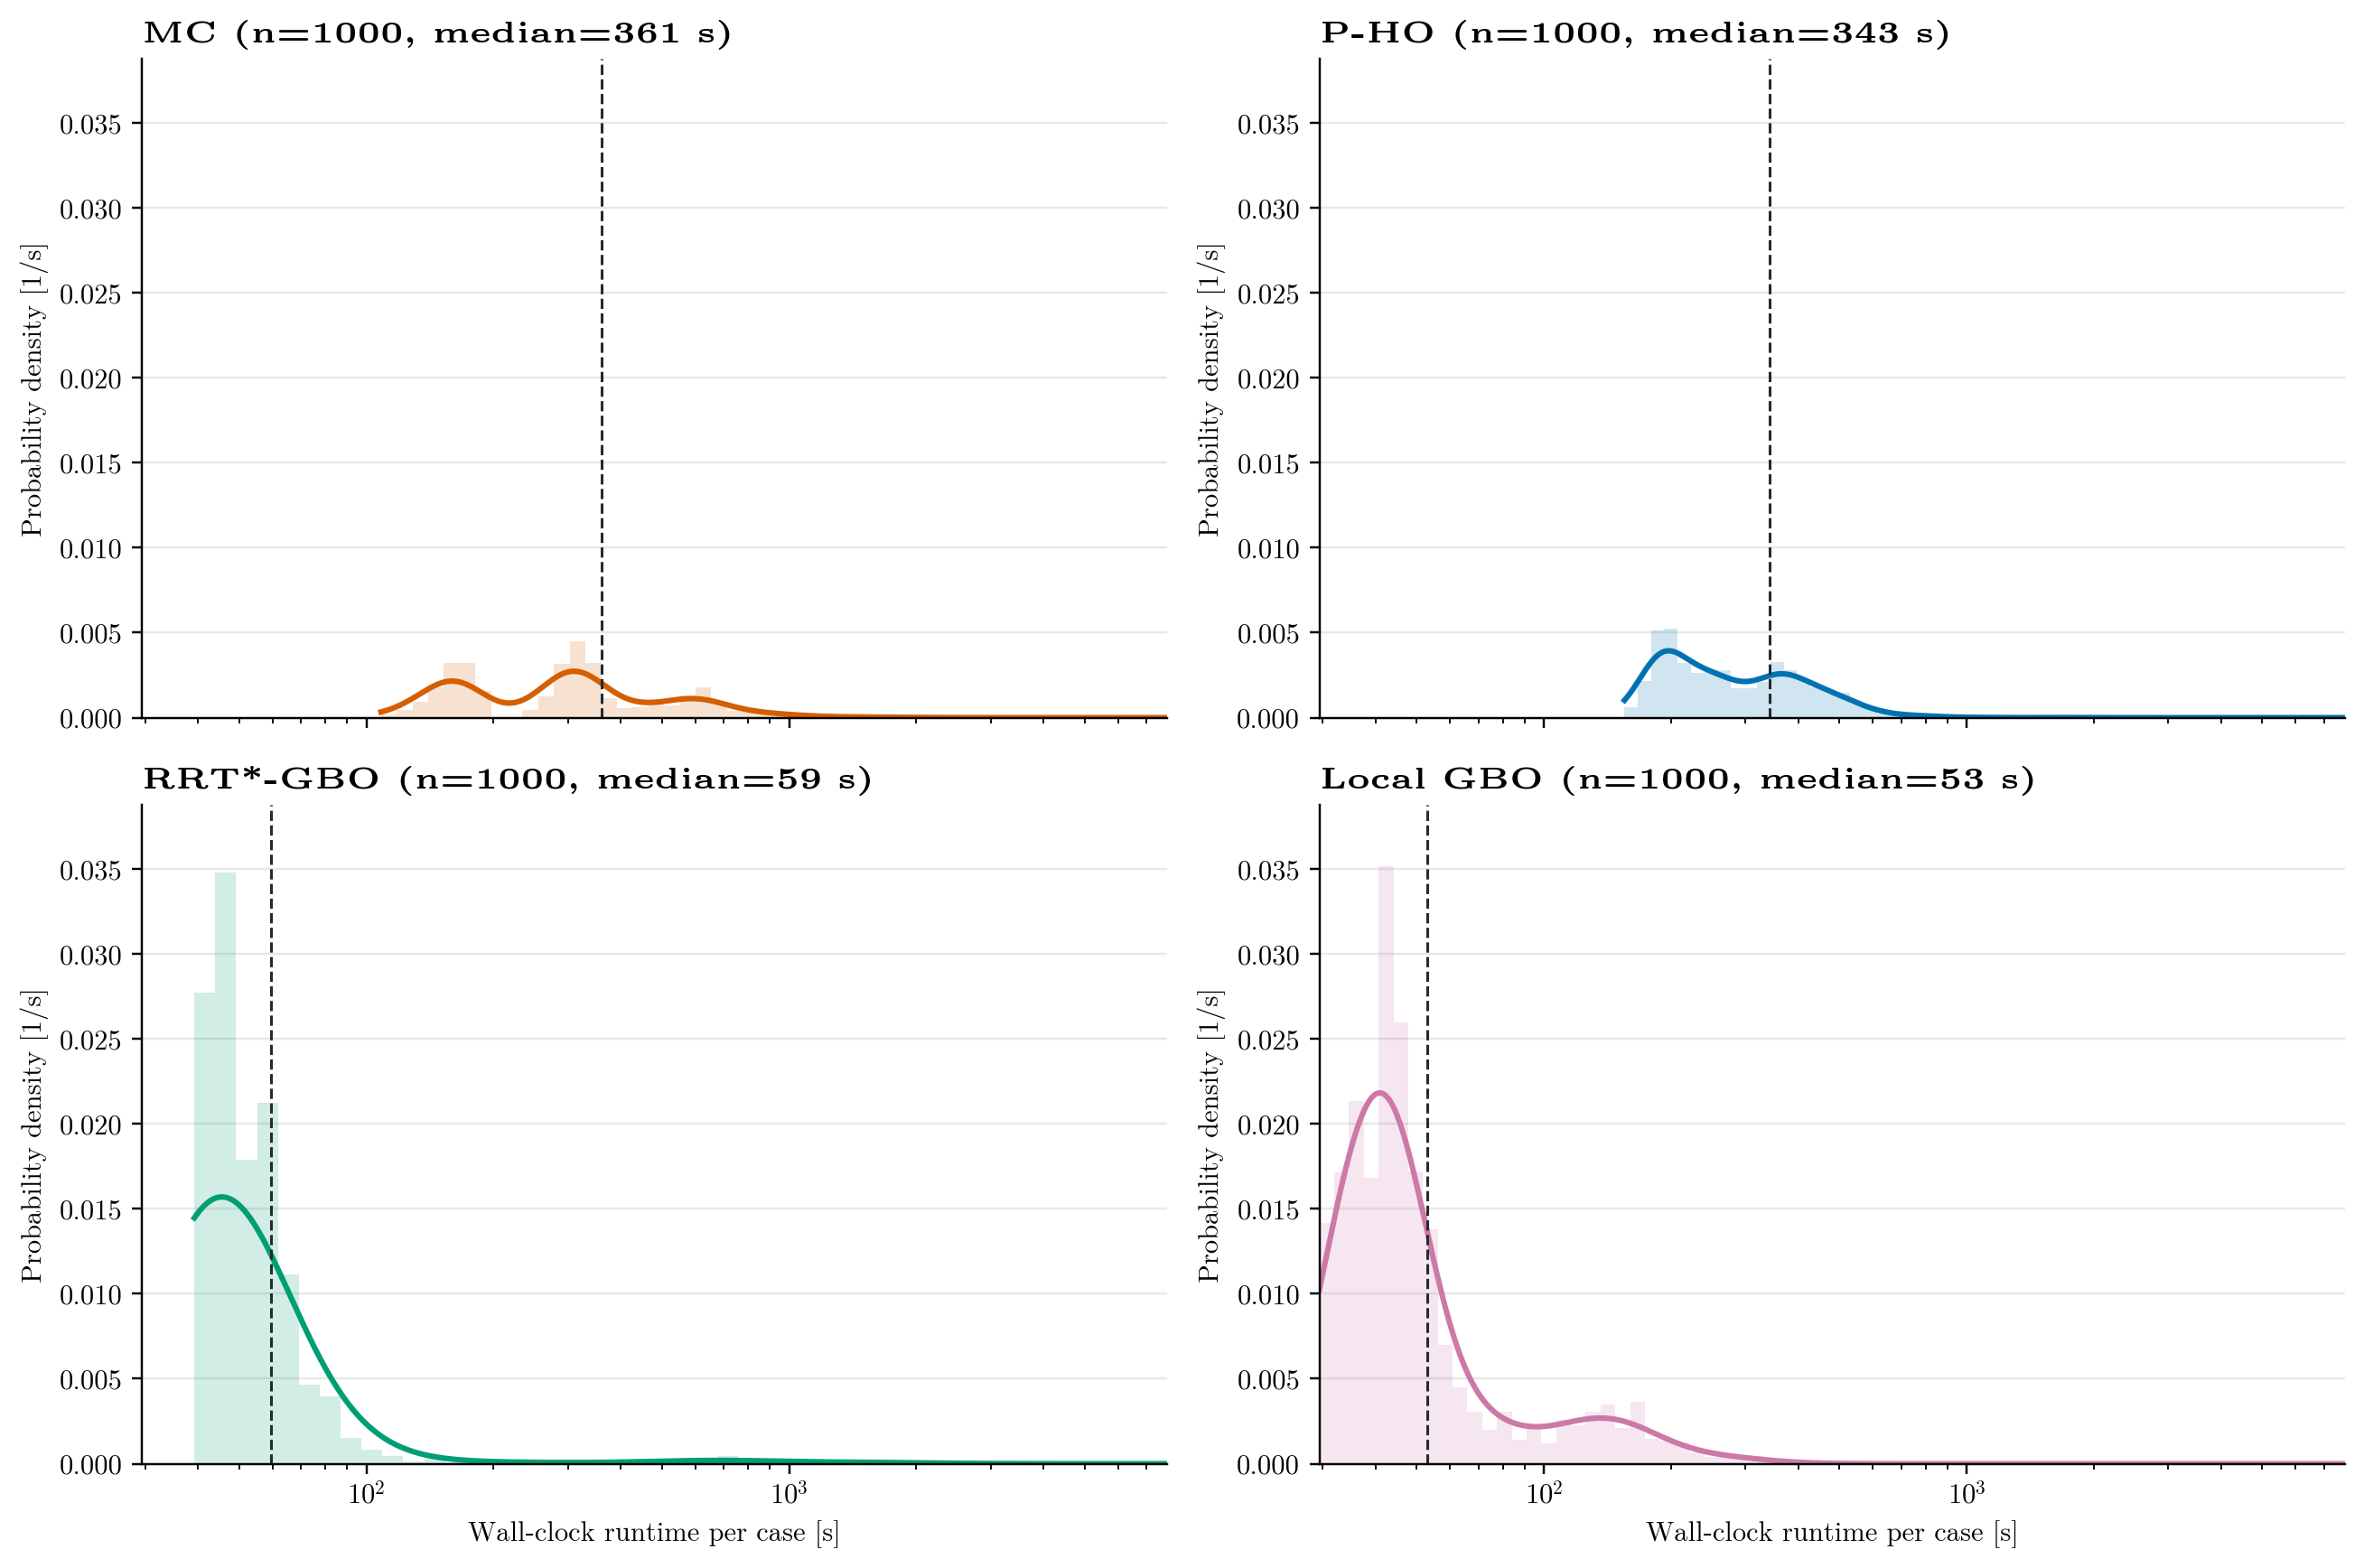
\includegraphics[width=\textwidth]{images/1000LUTRuns/runtime_distribution.png}
\caption{Distribution of wall-clock runtime per manipulator test case for the four algorithms. The dashed lines indicate the median runtime reported in the plot titles.}
\label{fig:manipulator-runtime-distribution}
\end{figure}
\todoX{Make the text on this success plots larger, or make only 2 plots per row}

\begin{figure}[htbp]
\centering
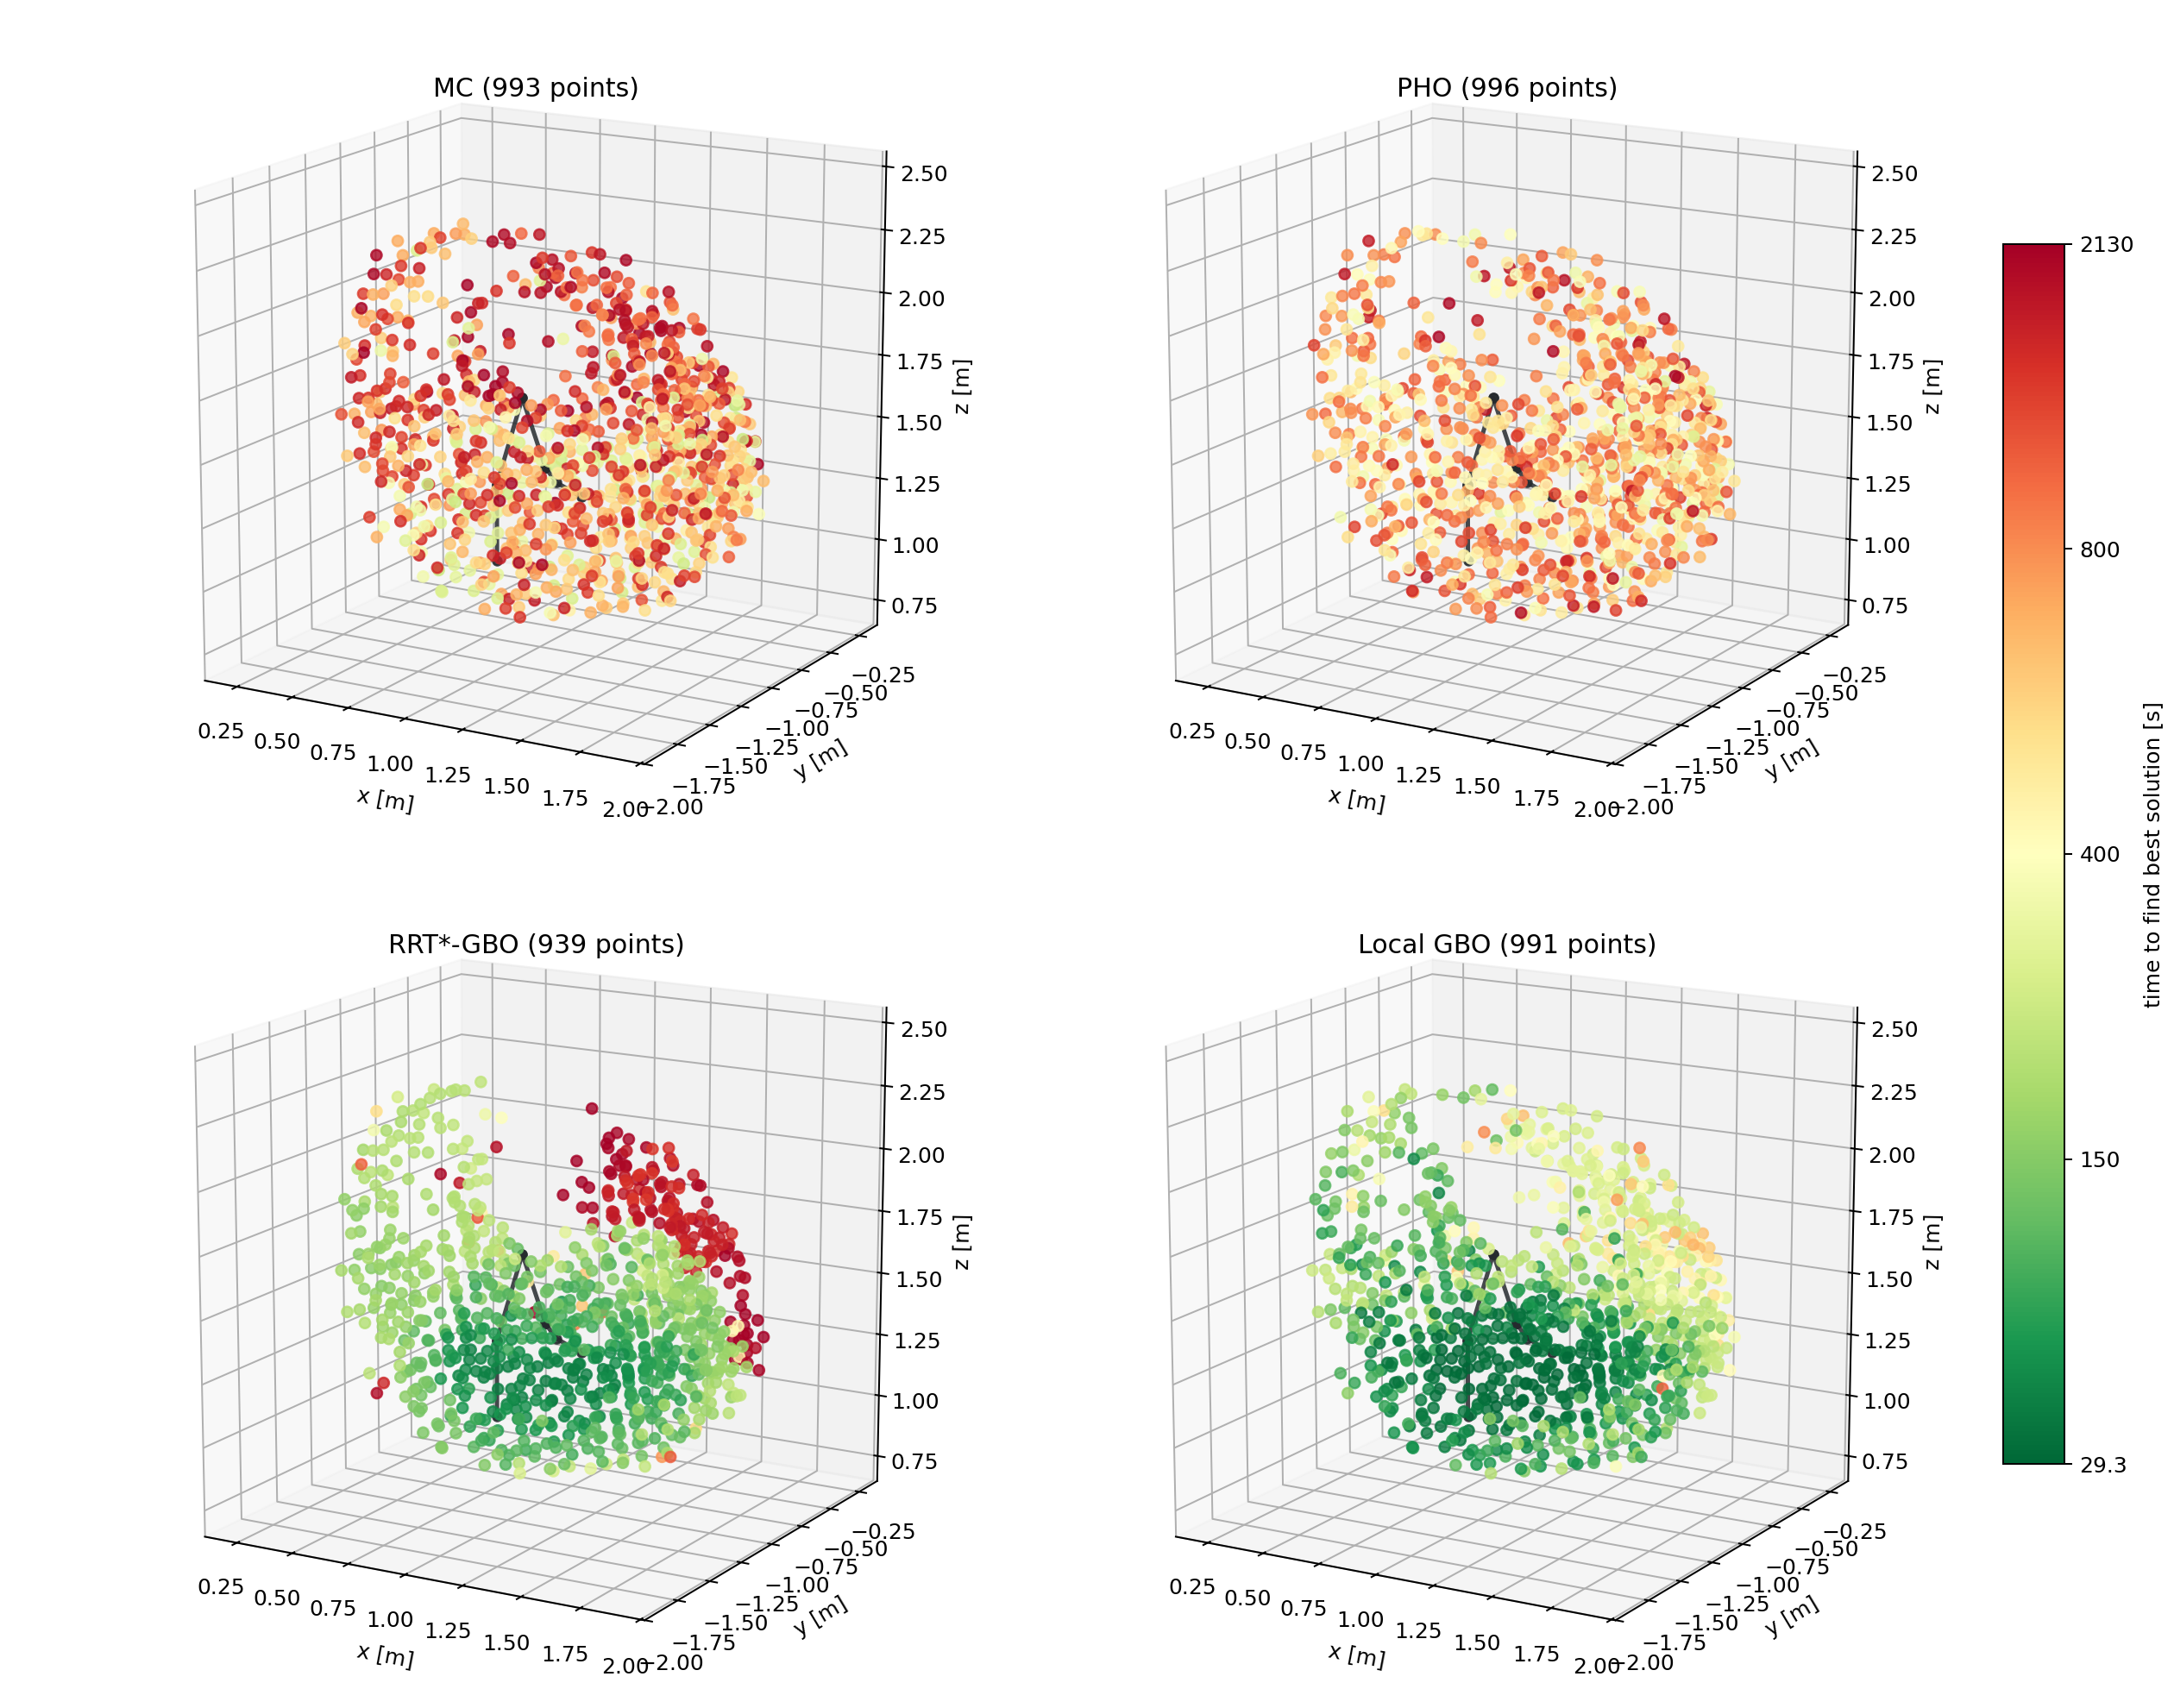
\includegraphics[width=\textwidth]{images/1000LUTRuns/arm7_success_point_cloud.png}
\caption{Spatial distribution of successful end-effector catch points for the four algorithms across the 1,000 manipulator test cases. The point colors encode the time required to find the best solution for each case.}
\label{fig:arm7-success-point-cloud}
\end{figure}

\begin{figure}[htbp]
\centering
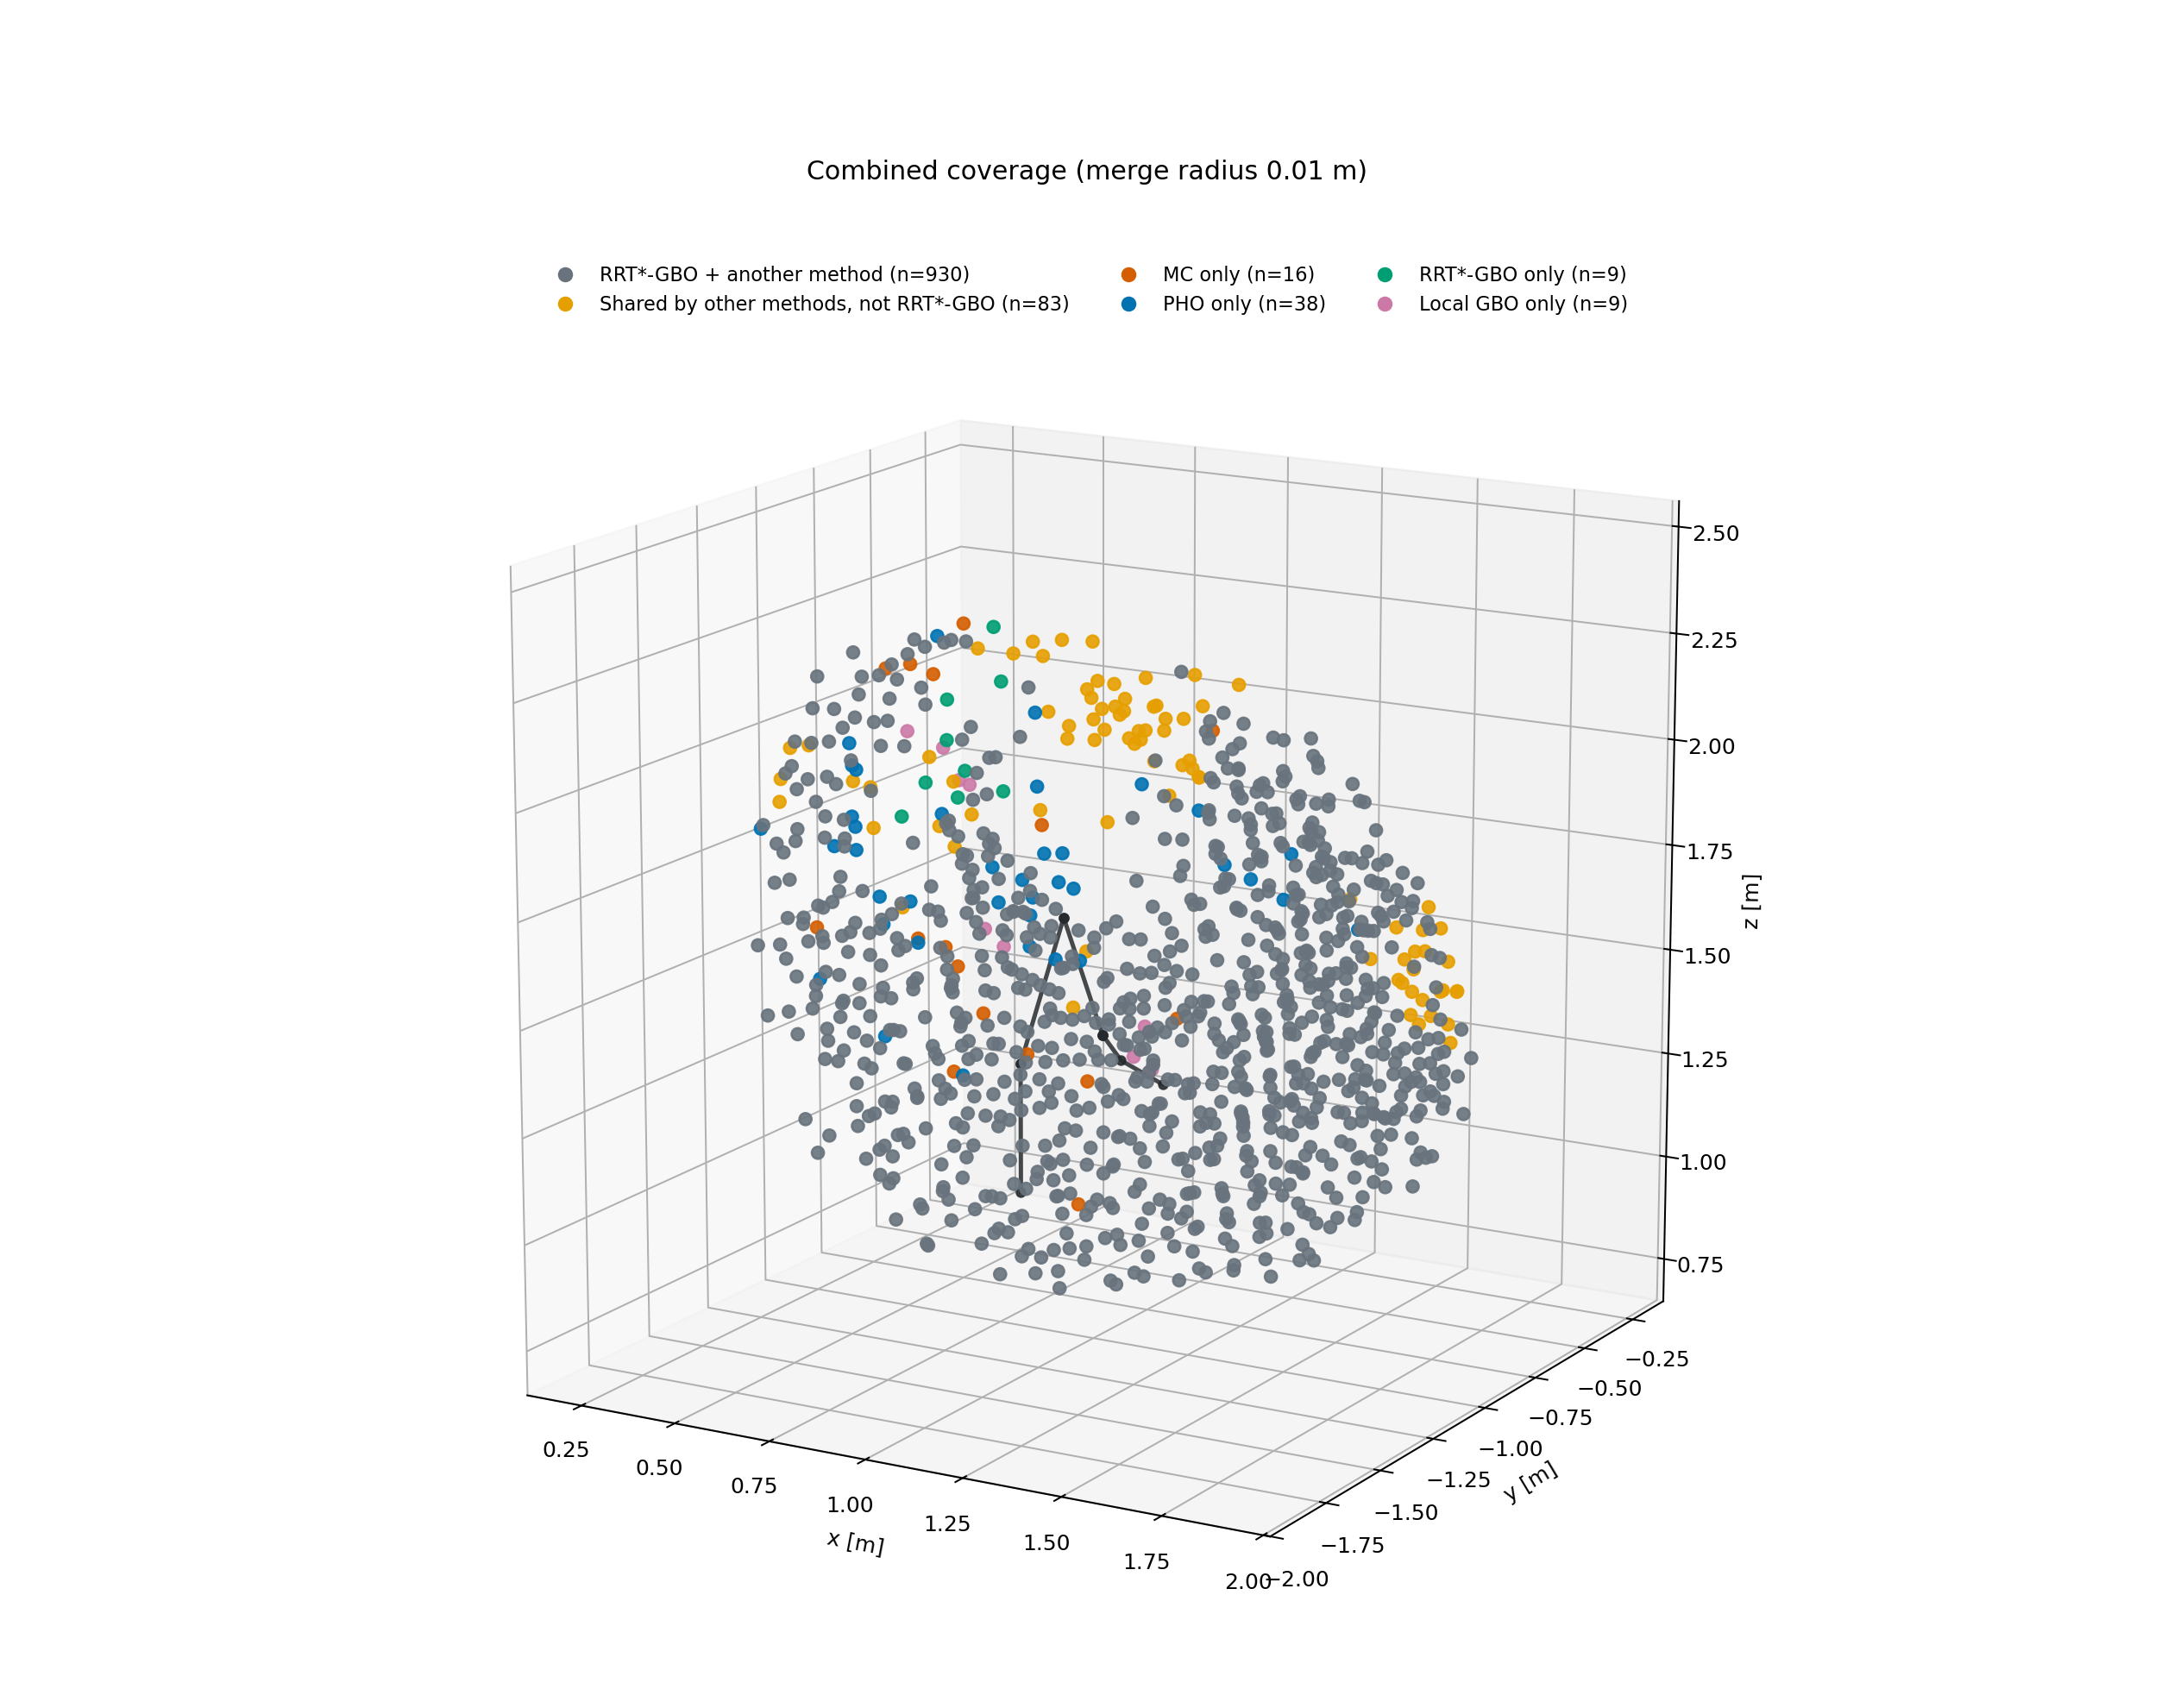
\includegraphics[width=\textwidth]{images/1000LUTRuns/arm7_success_point_cloud_combined_study.png}
\caption{Combined coverage of successful end-effector catch points. Points are grouped according to which algorithms produce a solution within the merge radius of $0.01\,\mathrm{m}$.}
\label{fig:arm7-combined-success-point-cloud}
\end{figure}

\begin{figure}[htbp]
\centering
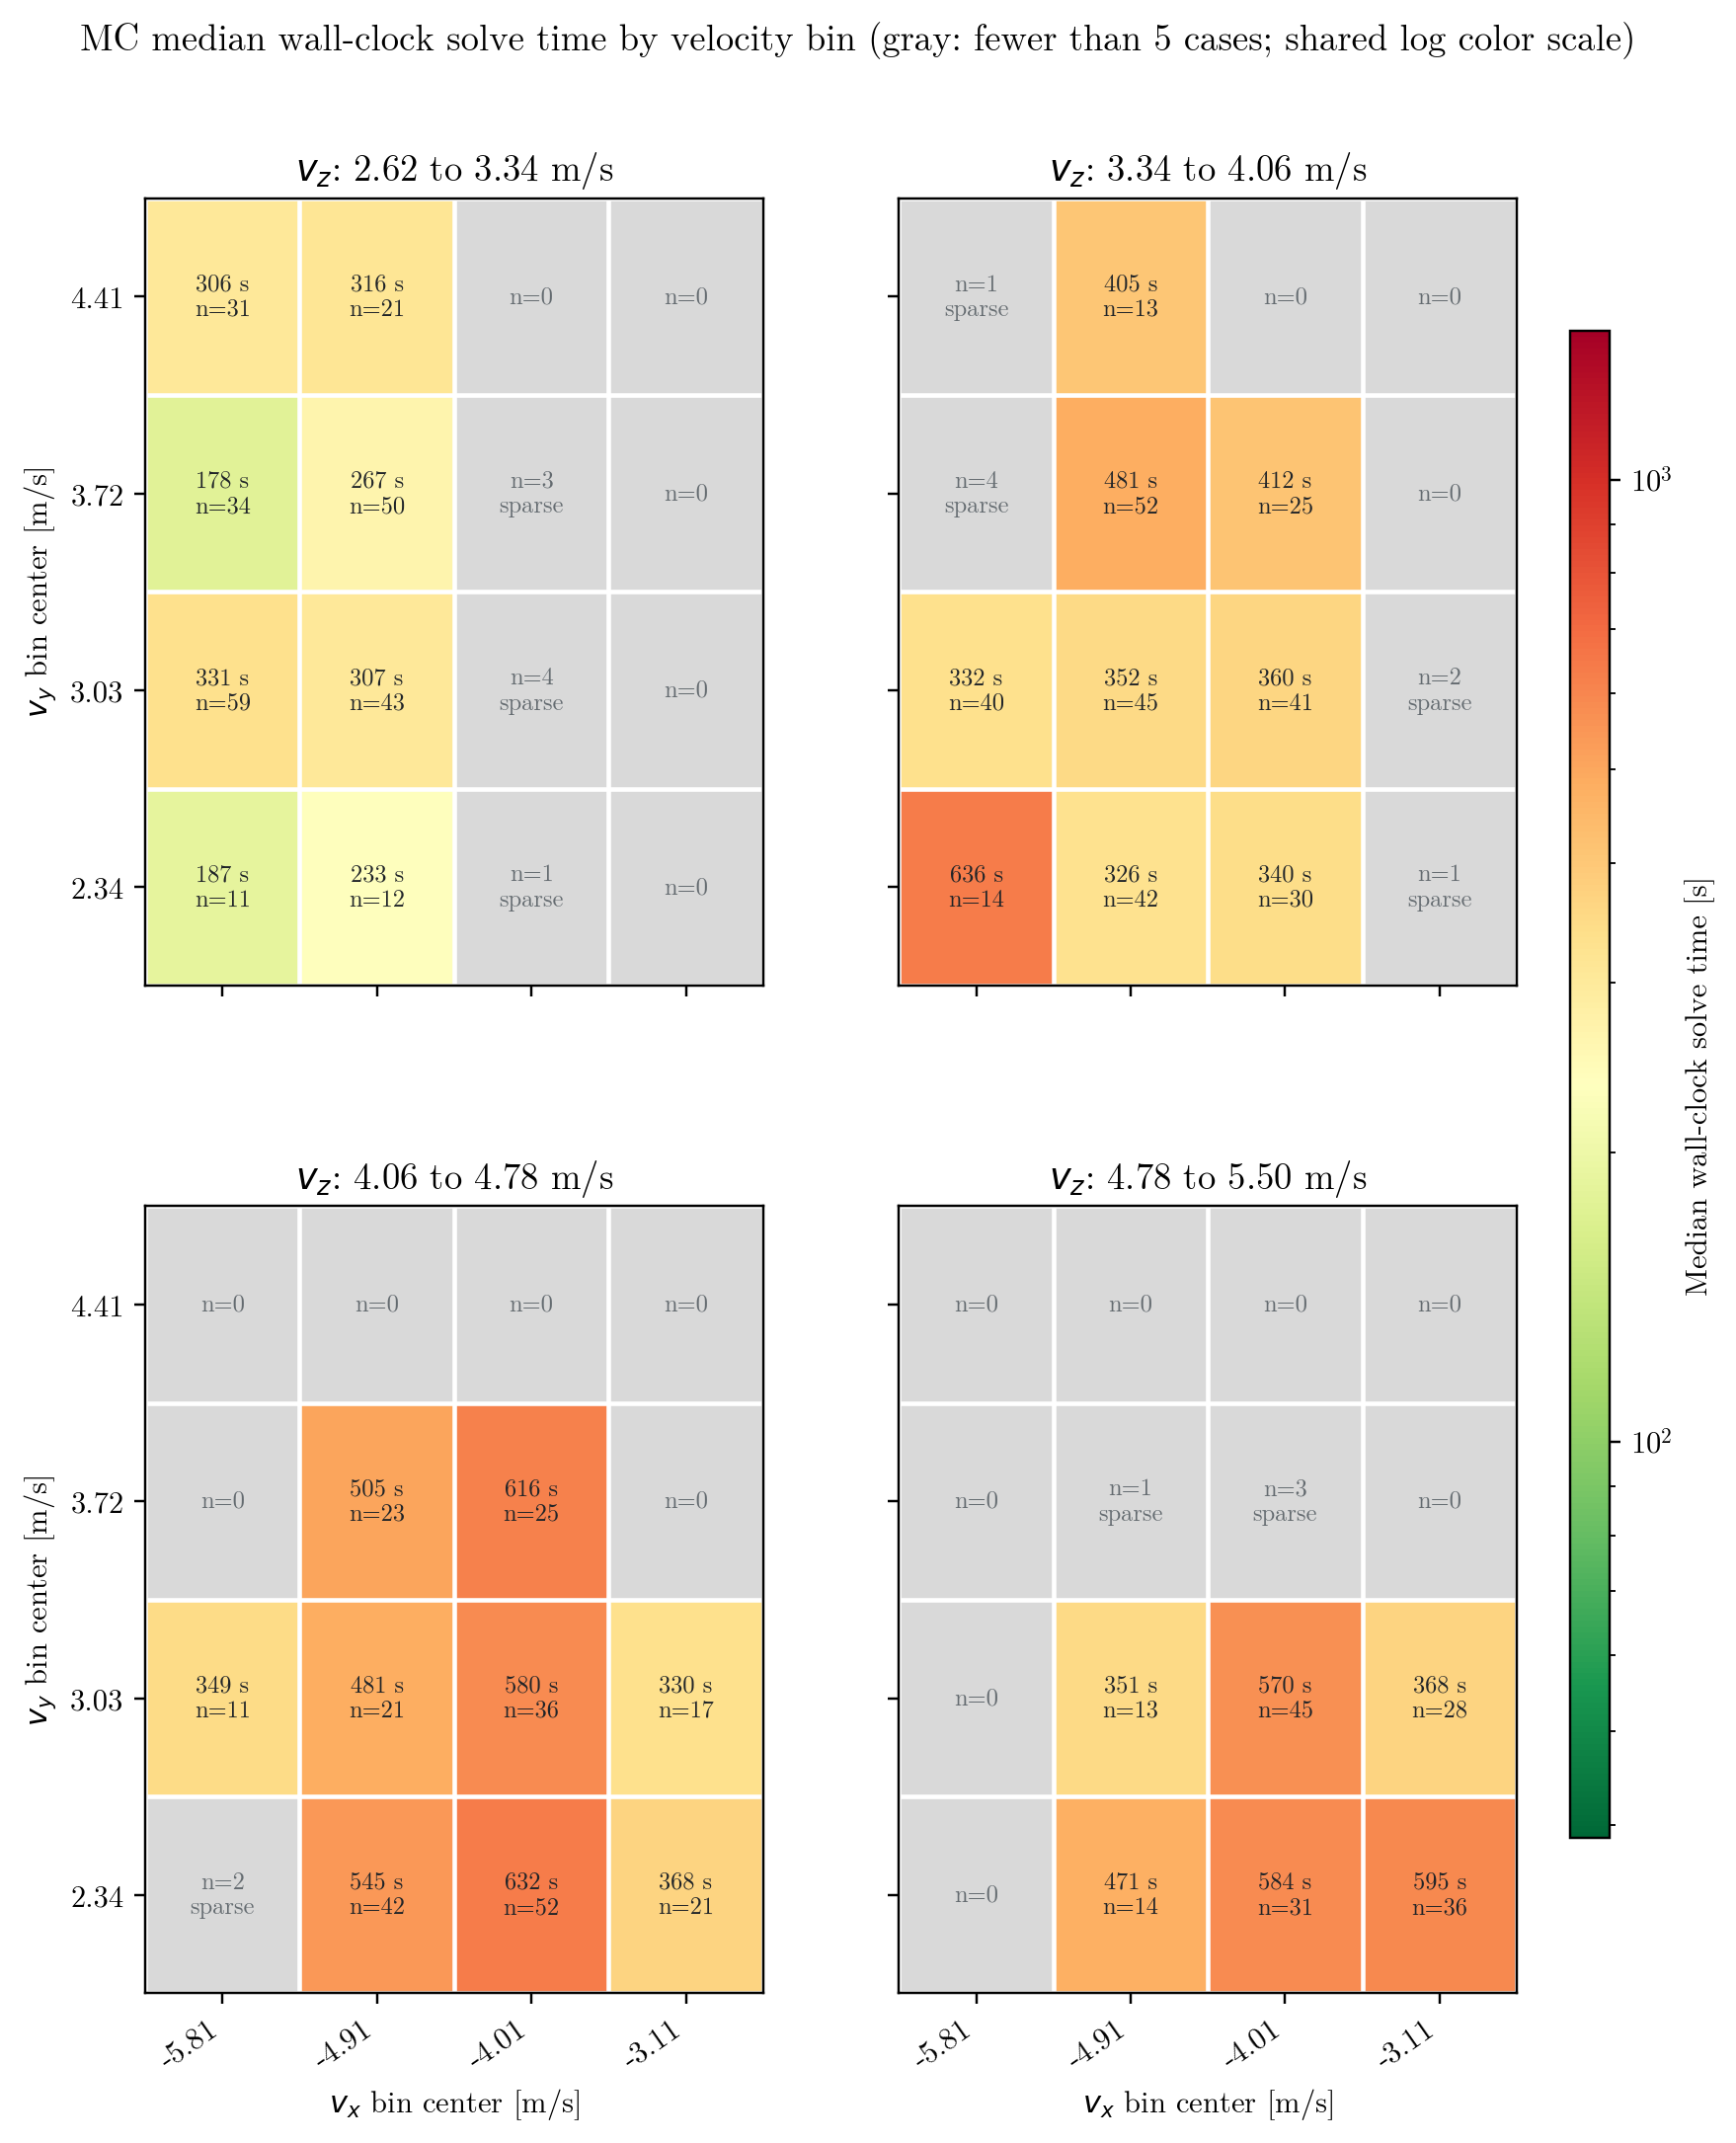
\includegraphics[width=\textwidth]{images/1000LUTRuns/runtime_velocity_heatmap_mc.png}
\caption{Runtime heatmap for MC over the 1,000 manipulator test cases, showing the relationship between computation time and initial velocity.}
\label{fig:runtime-velocity-heatmap-mc}
\end{figure}

\begin{figure}[htbp]
\centering
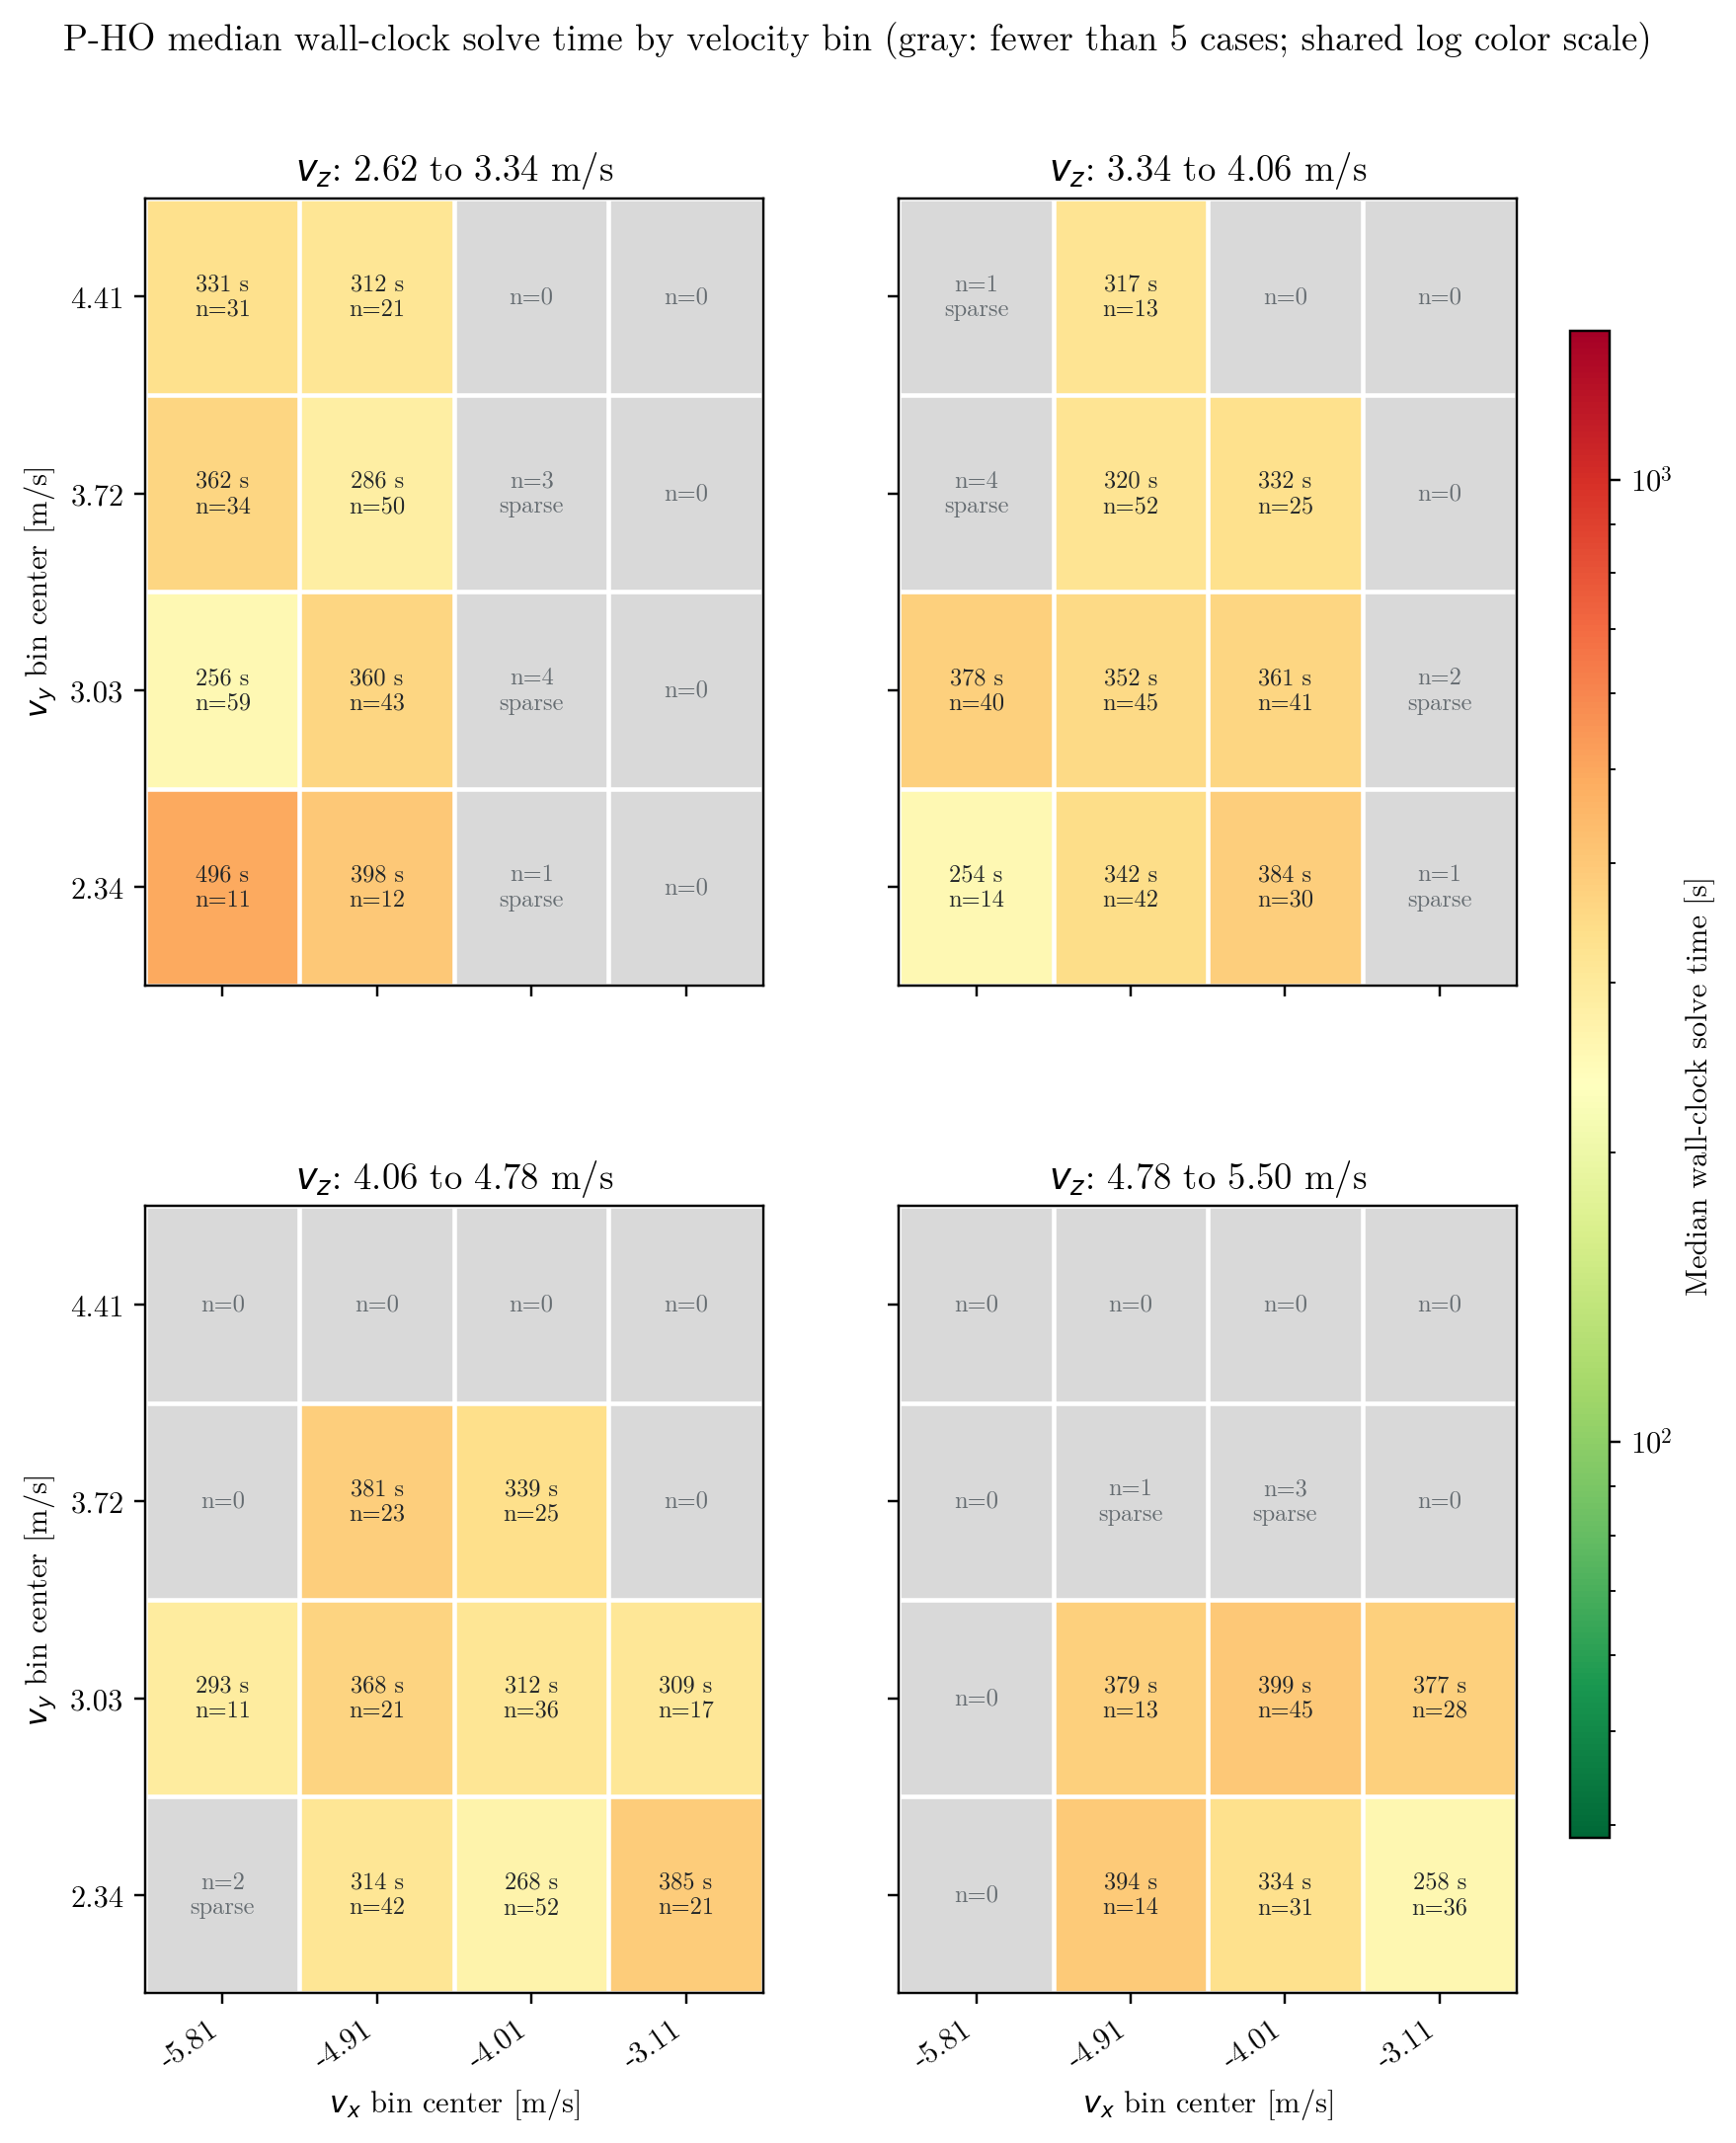
\includegraphics[width=\textwidth]{images/1000LUTRuns/runtime_velocity_heatmap_pho.png}
\caption{Runtime heatmap for P-HO over the 1,000 manipulator test cases, showing the relationship between computation time and initial velocity.}
\label{fig:runtime-velocity-heatmap-pho}
\end{figure}

\begin{figure}[htbp]
\centering
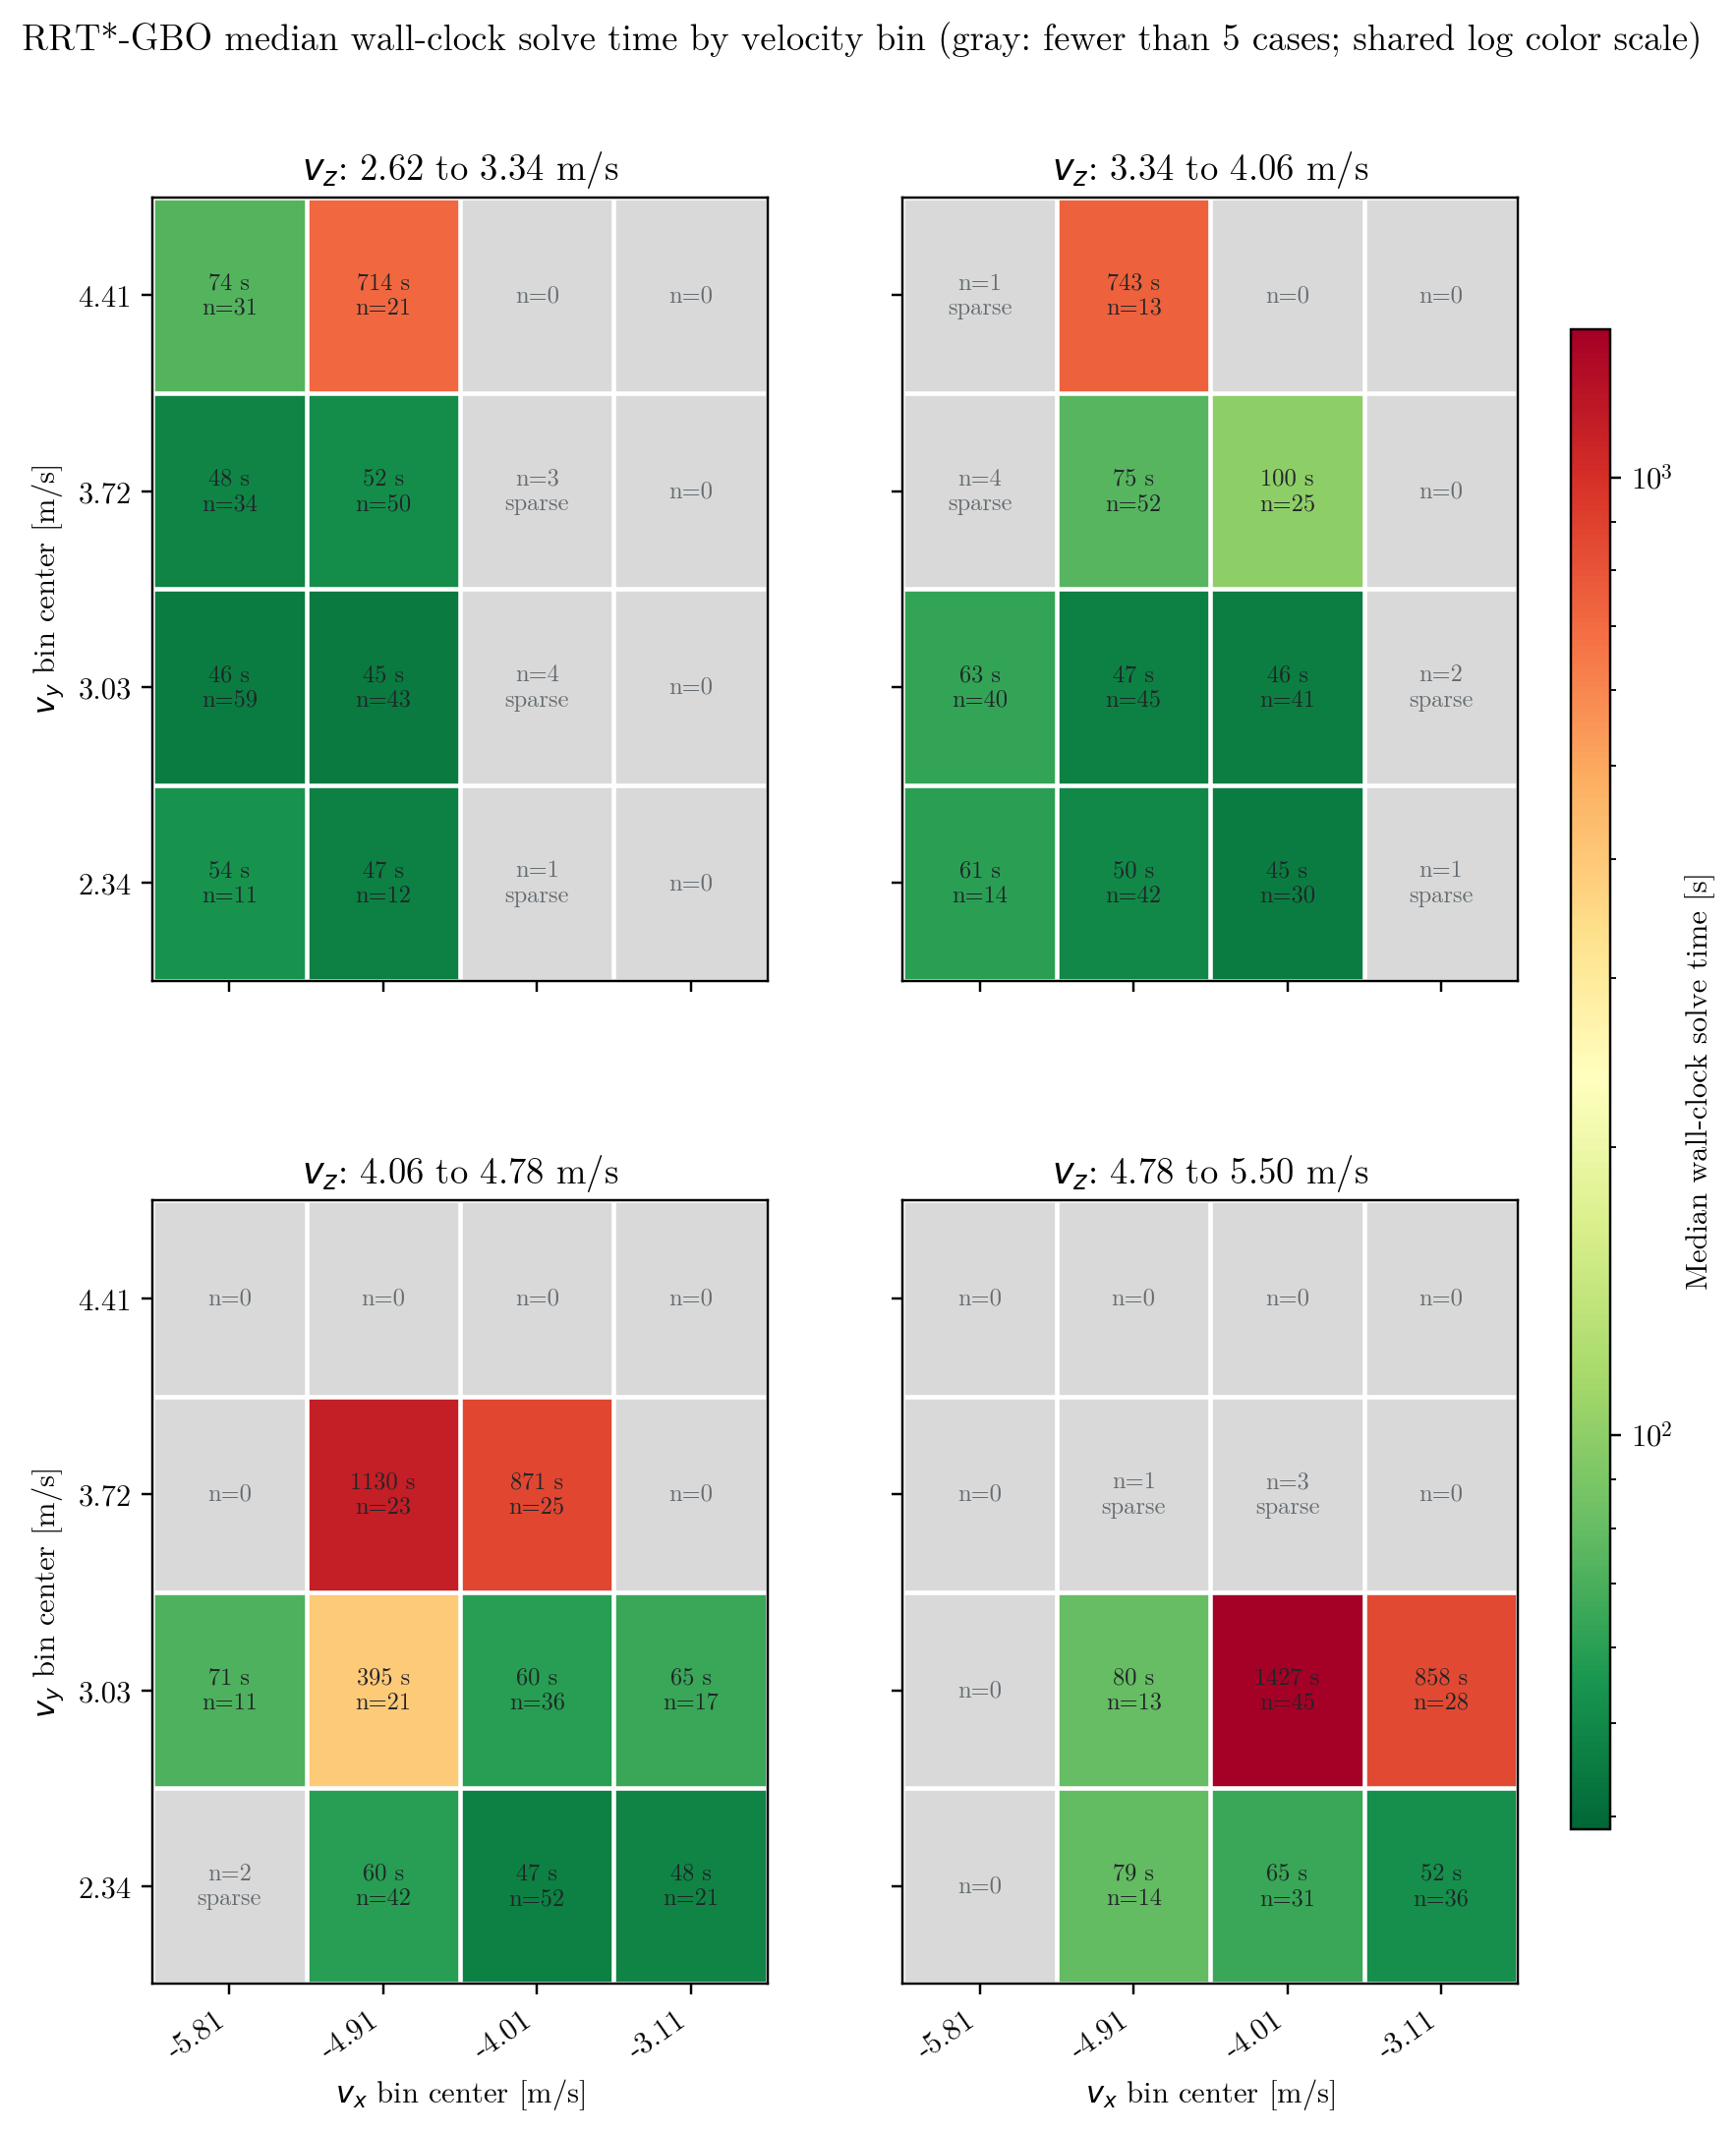
\includegraphics[width=\textwidth]{images/1000LUTRuns/runtime_velocity_heatmap_rrt_star_gbo.png}
\caption{Runtime heatmap for RRT*-GBO over the 1,000 manipulator test cases, showing the relationship between computation time and initial velocity.}
\label{fig:runtime-velocity-heatmap-rrt-star-gbo}
\end{figure}

\begin{figure}[htbp]
\centering
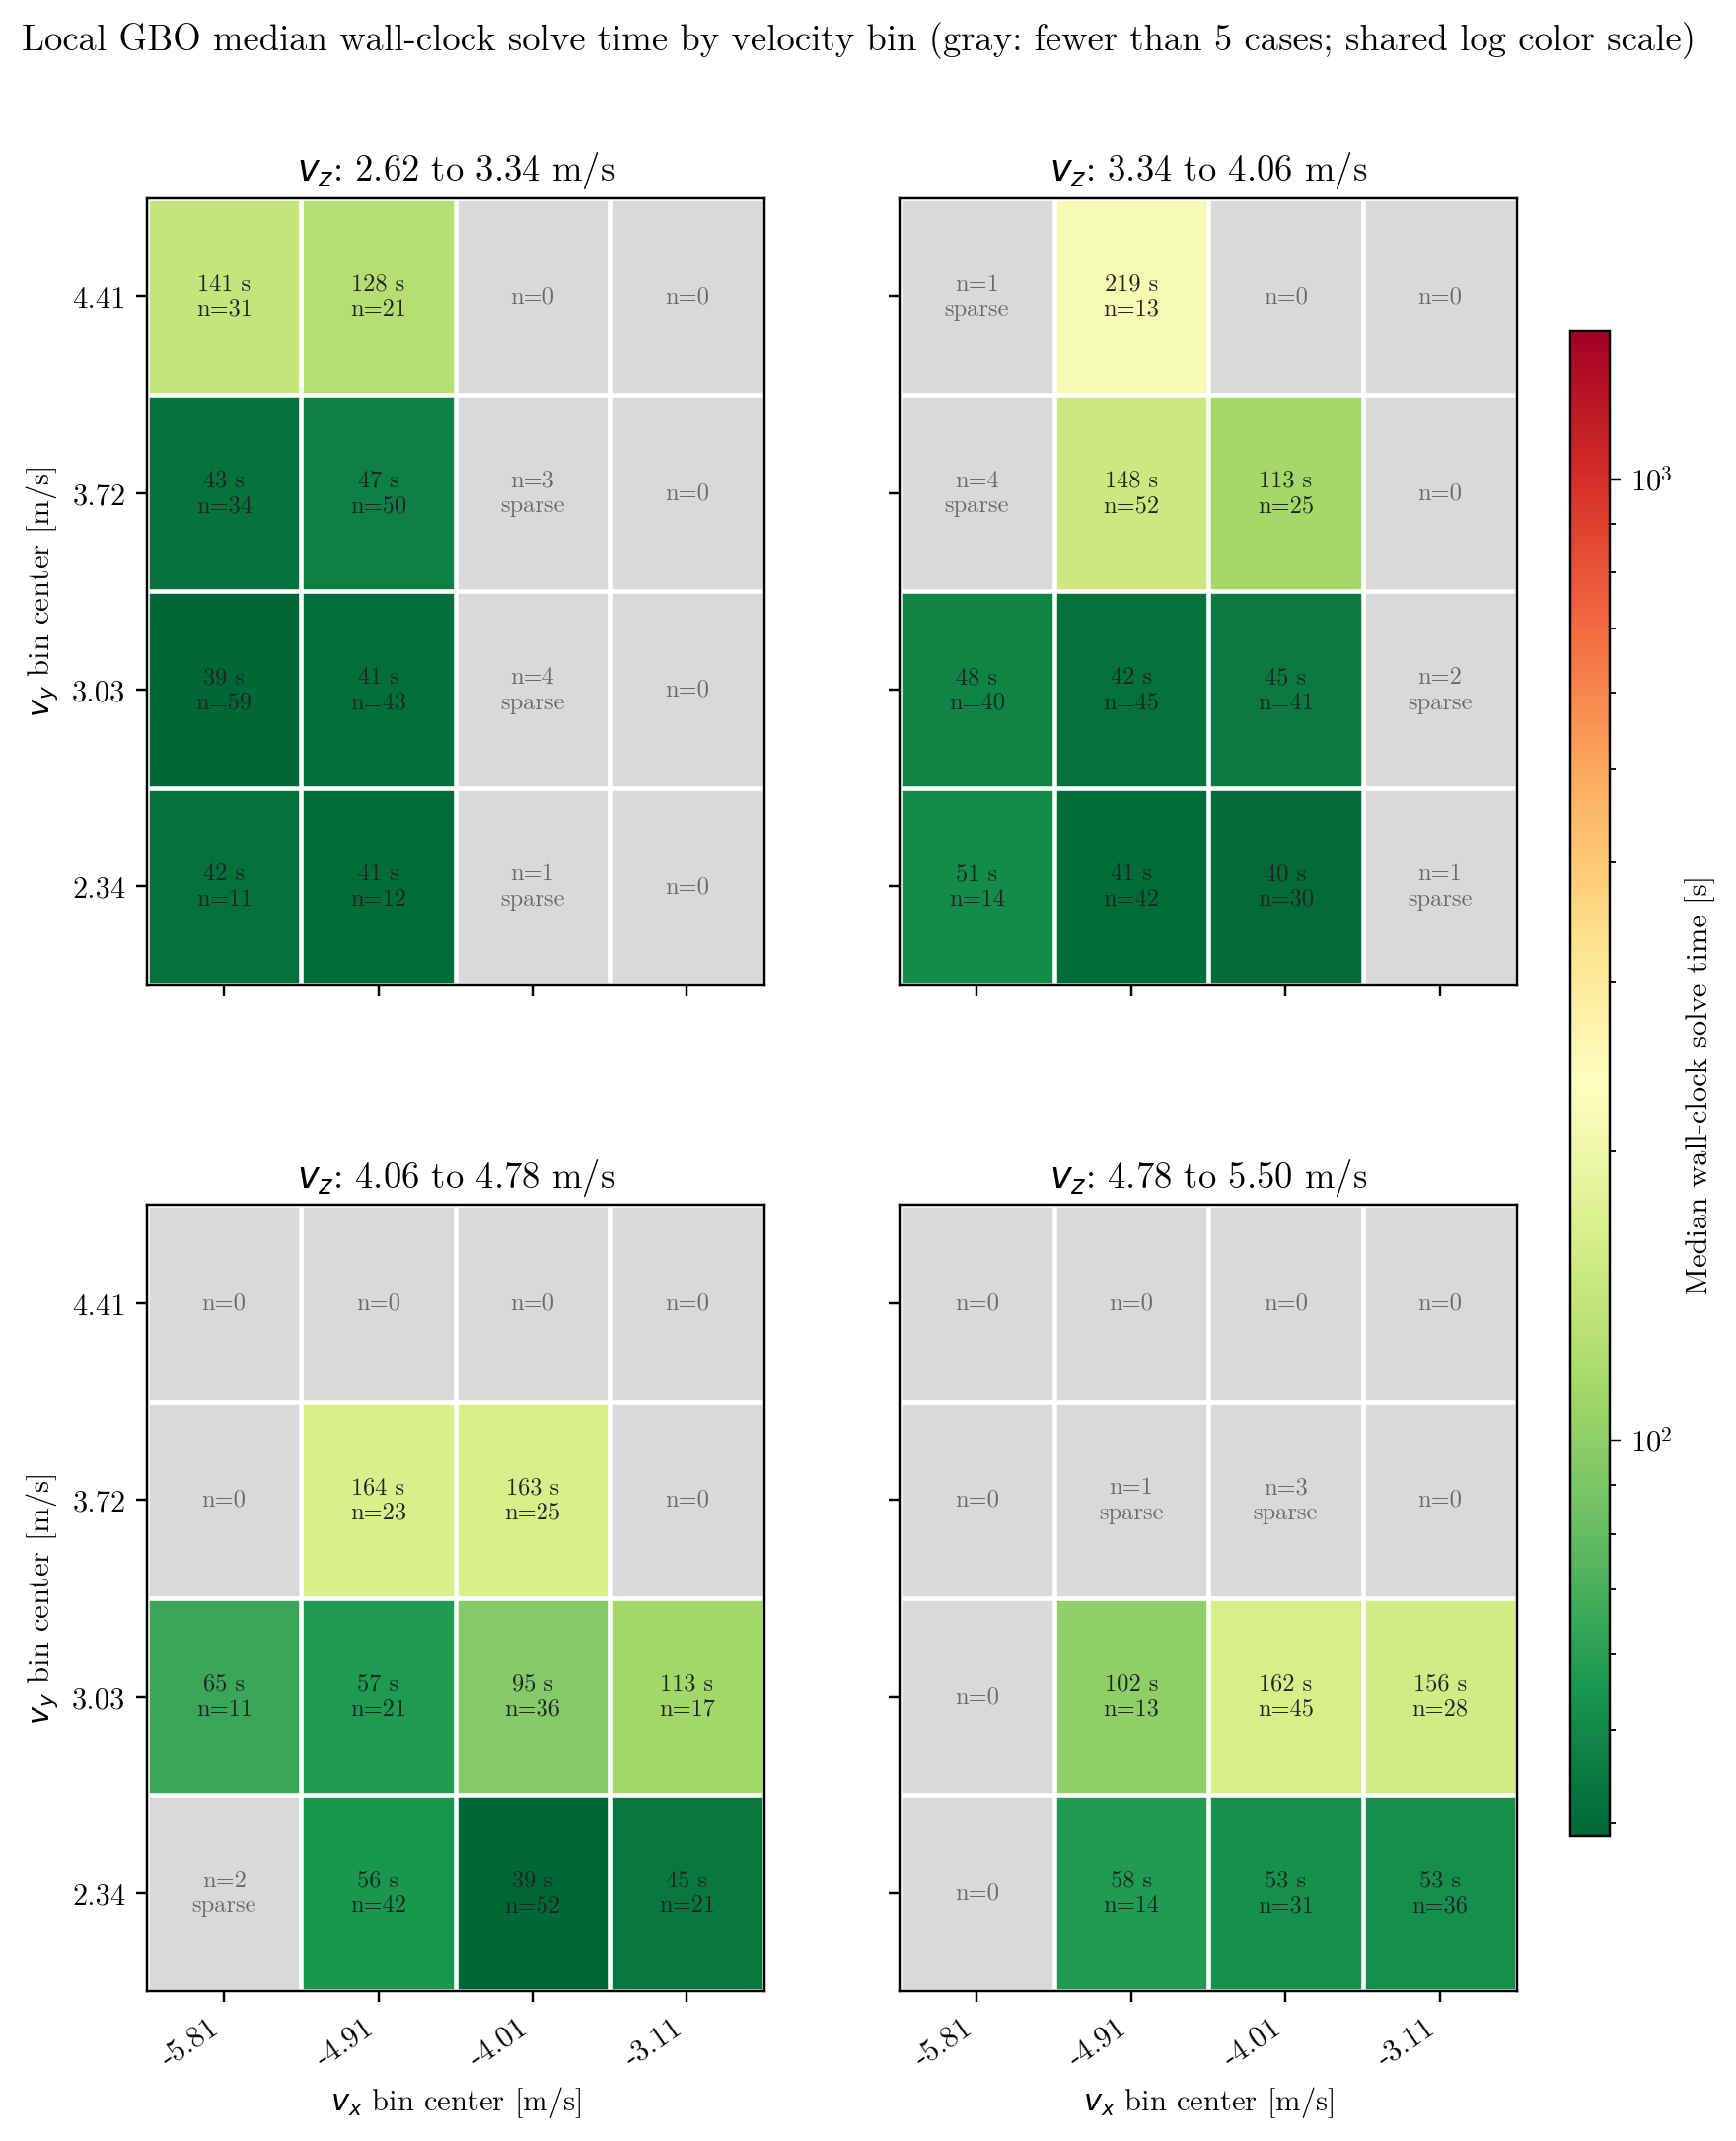
\includegraphics[width=\textwidth]{images/1000LUTRuns/runtime_velocity_heatmap_local_gbo.png}
\caption{Runtime heatmap for Local GBO over the 1,000 manipulator test cases, showing the relationship between computation time and initial velocity.}
\label{fig:runtime-velocity-heatmap-local-gbo}
\end{figure}




\subsection{100-Lut Runs Global Landscape Evaluation Set}

\begin{table}[ht]
\centering
\caption{Best costs versus the \ac{LUT} reference among the selected 100 \ac{LUT} rows; differences within 0.5\% are equivalent.}
\label{tab:100-global-fcv-cost-comparison}
\begin{tabular}{lrrrr}
\hline
Algorithm & Better & Equivalent & Worse \\
\hline
MC & 1 & 55 & 0 \\
P-HO & 1 & 55 & 0 \\
RRT*-GBO & 1 & 55 & 0\\
Local GBO & 1 & 54 & 1 \\
\hline
\end{tabular}
\end{table}


\begin{table}[ht]
\centering
\caption{Distinct successful local minima for the selected \ac{LUT} cases with finite results from all four methods. Costs within 0.5\% of a group minimum are merged; $\times n$ gives the number of solutions in each group.}
\label{tab:100-global-local-minima-by-case}
\small
\begin{tabular}{r p{0.18\textwidth} p{0.18\textwidth} p{0.18\textwidth} p{0.18\textwidth}}
\hline
\ac{LUT} row & MC & P-HO & RRT*-GBO & Local GBO \\
\hline
1 & 2.824357 ($\times$110) & 2.824357 ($\times$28) & 2.824357 & 2.824357 \\
56 & 0.243846 ($\times$182) & 0.243846 ($\times$32) & 0.243846 & 0.243846 \\
93 & 2.017878 ($\times$3) & 2.017878 ($\times$23) & 2.017878 & 2.017878 \\
185 & 0.196607 ($\times$158) & 0.196607 ($\times$45) & 0.196607 & 0.196607 \\
204 & 0.497014 ($\times$74) & 0.497009 ($\times$67) & 0.497009 & 0.497009 \\
241 & 0.618631 ($\times$89), 3.404011 ($\times$65) & 0.618631 ($\times$33) & 0.618631 & 0.618631 \\
333 & 0.826499 ($\times$167) & 0.826499 ($\times$35) & 0.826499 & 0.826499 \\
388 & 0.395060 ($\times$133) & 0.395058 ($\times$44) & 0.395058 & 0.395058 \\
554 & 0.008523 ($\times$140) & 0.008523 ($\times$17) & 0.008523 & 0.008523 \\
646 & 2.322030 ($\times$154) & 2.322030 ($\times$32) & 2.322030 & 2.322030 \\
941 & 3.384427 ($\times$72) & 3.384426 ($\times$20) & 3.384426 & 3.384426 \\
1014 & 0.031773 ($\times$88), 3.040450 & 0.031773 ($\times$13) & 0.031773 & 0.031773 \\
1217 & 0.359450 ($\times$45) & 0.359449 ($\times$14) & 0.359449 & 0.359449 \\
1383 & 0.454051 ($\times$38), 0.462116, 0.517761, 0.533384 & 0.454048 ($\times$25) & 0.454048 & 0.454048 \\
1401 & 1.065105 ($\times$8) & 1.065100 ($\times$12) & 1.065100 & 1.065100 \\
1585 & 0.380868 ($\times$21) & 0.380867 ($\times$10) & 0.380867 & 0.380867 \\
1659 & 0.040879 ($\times$42), 0.041151 ($\times$2), 0.041467, 0.162265, 0.167889 ($\times$2), 0.169325, 0.170625 & 0.040879 ($\times$6) & 0.040879 & 0.040879 \\
1678 & 0.811470 ($\times$38) & 0.811470 ($\times$26) & 0.811470 & 0.811470 \\
1751 & 0.038230 ($\times$72) & 0.038230 ($\times$33) & 0.038230 & 0.038230 \\
1788 & 1.418019 ($\times$116) & 1.418018 ($\times$36) & 1.418018 & 1.418018 \\
\hline
\end{tabular}
\end{table}

\begin{table}[ht]
\centering
\caption{Representative unique terminal configurations for \ac{LUT} row 241.}
\label{tab:mc-local-minima-row-241}
\begin{tabular}{|r|r|r|r|r|r|r|r|}
\hline
\multicolumn{7}{|c|}{$\theta(t_f)$ [deg]} & $J$ \\
\hline
9 & 22 & 19 & -83 & -15 & -5 & 38 & 0.619 \\
66 & -34 & 8 & -78 & -72 & -3 & -5 & 3.404 \\
\hline
\end{tabular}
\end{table}

\begin{table}[ht]
\centering
\caption{Representative unique terminal configurations for \ac{LUT} row 1659.}
\label{tab:mc-local-minima-row-1659}
\begin{tabular}{|r|r|r|r|r|r|r|r|}
\hline
\multicolumn{7}{|c|}{$\theta(t_f)$ [deg]} & $J$ \\
\hline
47 & 15 & 71 & -99 & 82 & 49 & -45 & 0.041 \\
56 & 6 & 78 & -90 & 47 & 3 & -9 & 0.162 \\
\hline
\end{tabular}
\end{table}

\todoX{probably remove the limit dashed lines on all except the normalized plot. cant see.}

\begin{figure}[htbp]
\centering
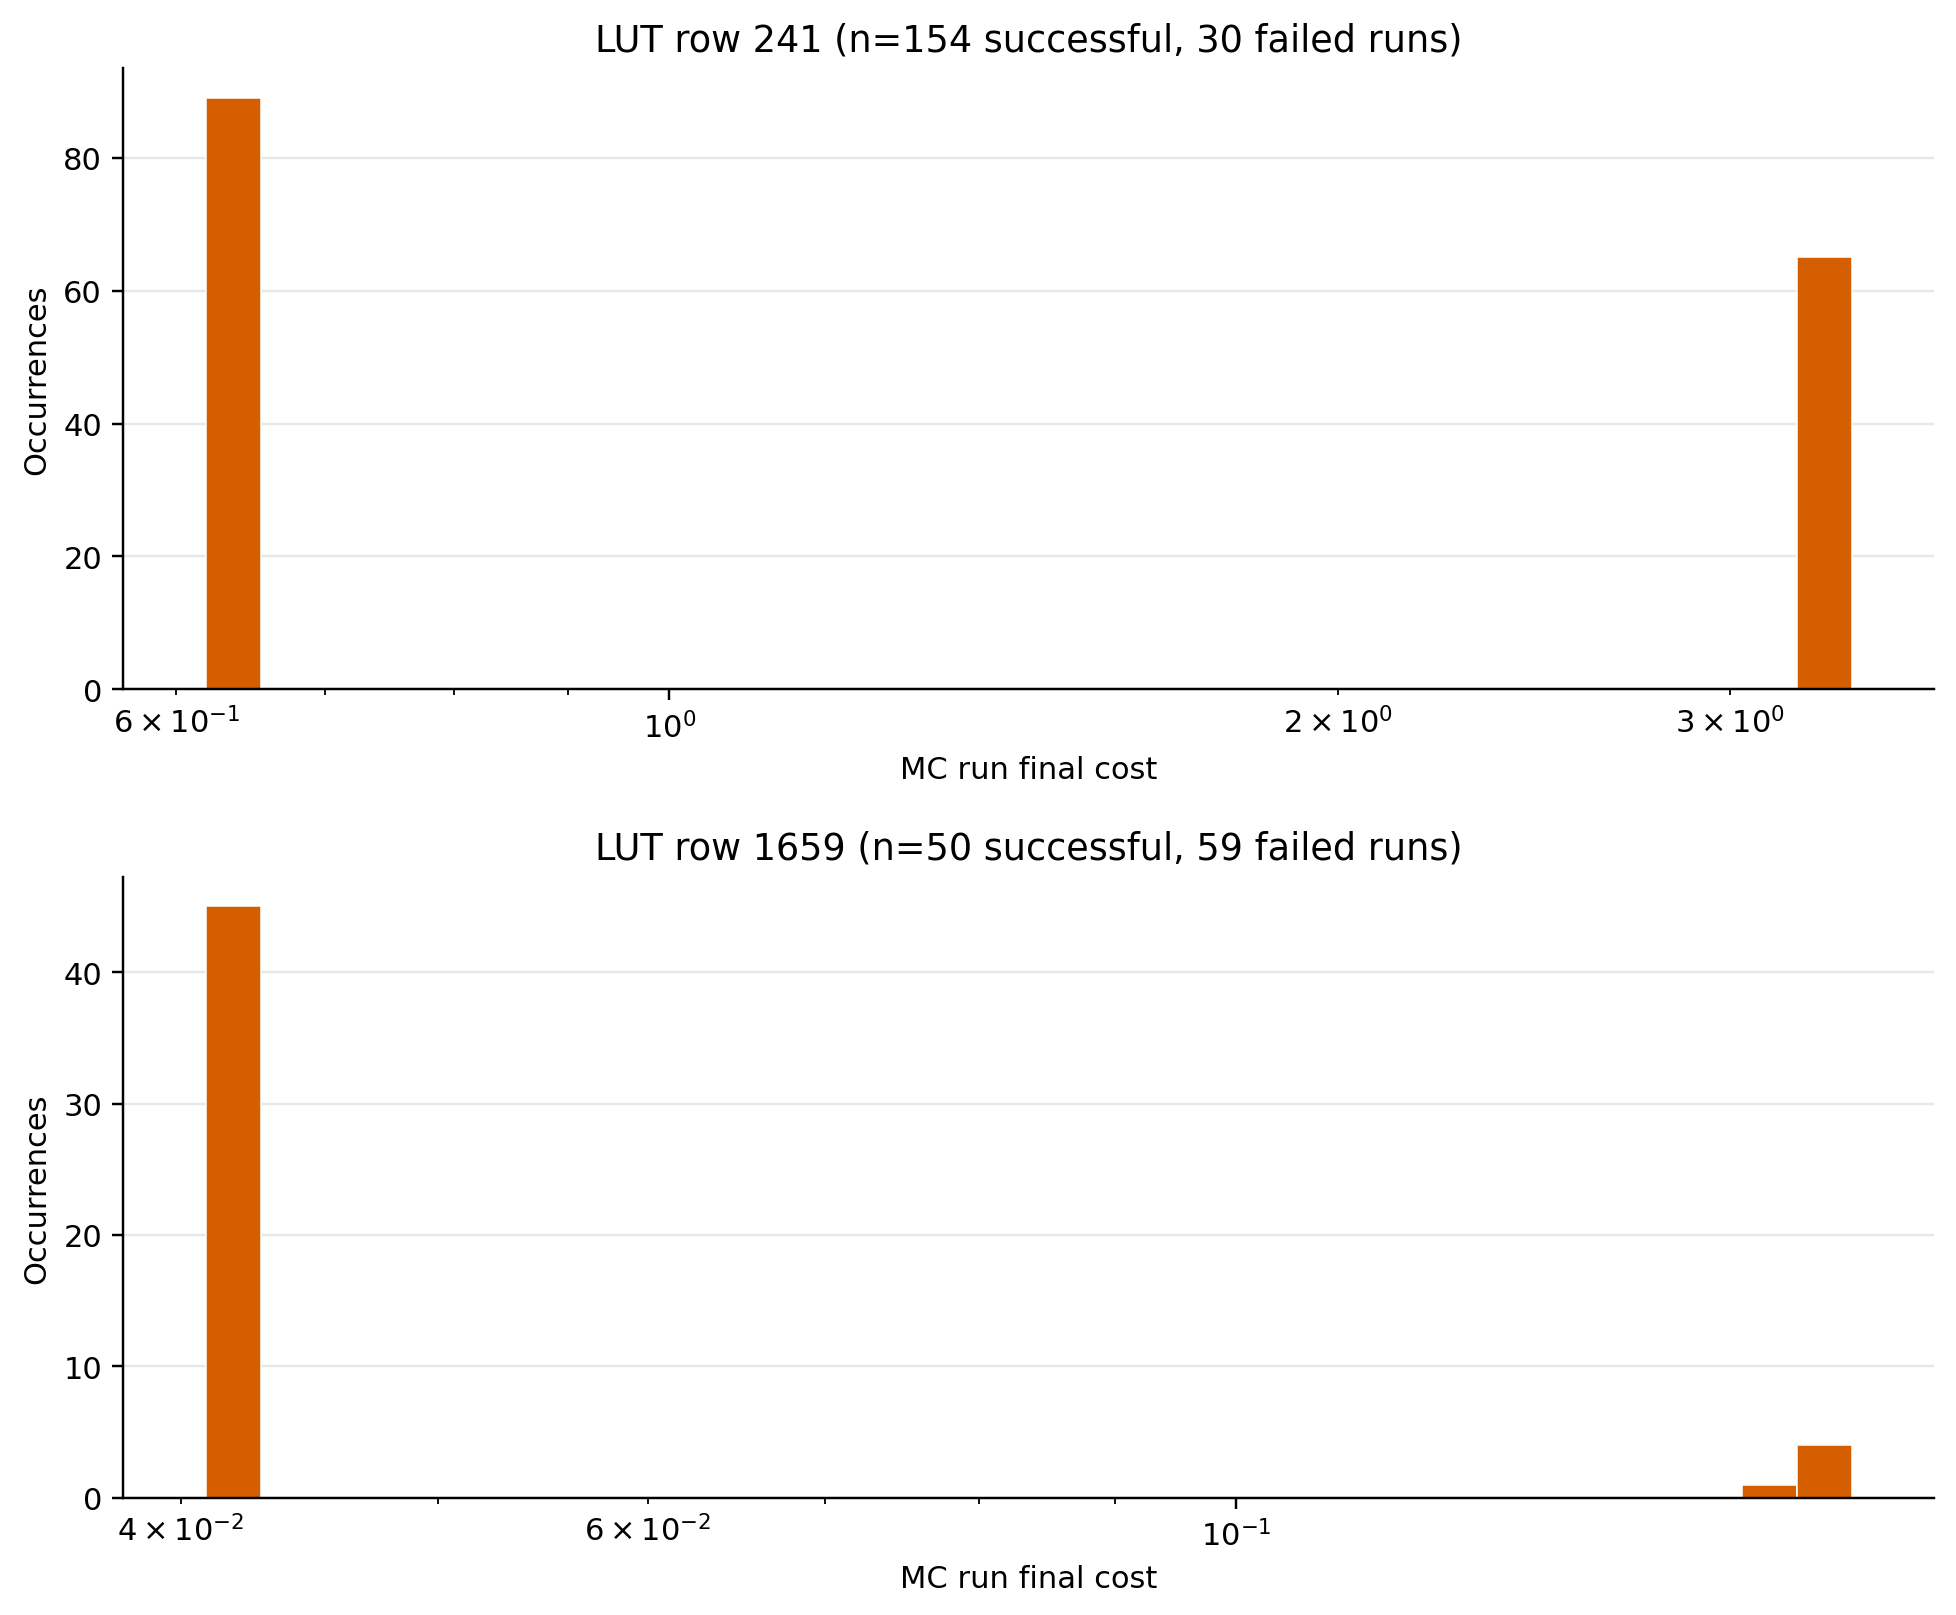
\includegraphics[width=\textwidth]{images/100GlobalRuns/mc_local_minima_rows_241_1659.png}
\caption{Distributions of the distinct final costs obtained by MC for \ac{LUT} rows 241 and 1659. The plots show the frequency of the two observed local-minimum groups among successful runs.}
\label{fig:mc-local-minima-distributions}
\end{figure}

\begin{figure}[htbp]
\centering
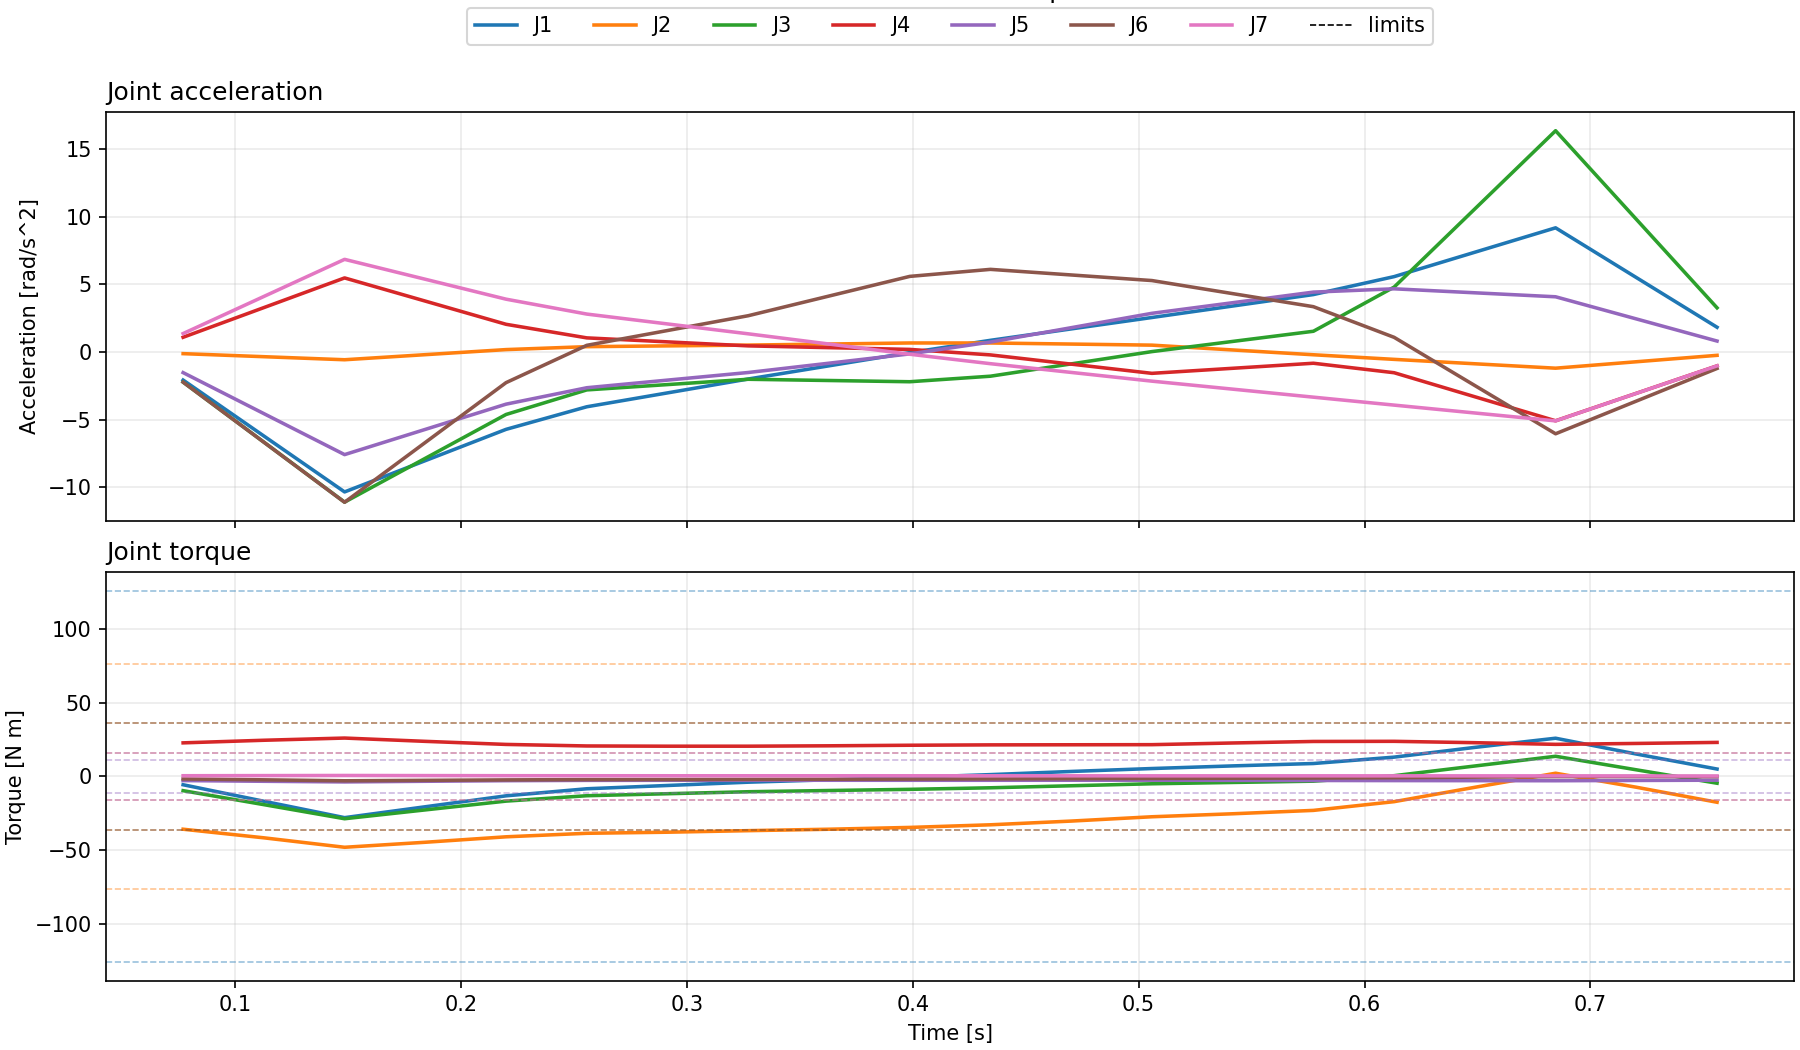
\includegraphics[width=\textwidth]{images/100GlobalRuns/row241_mc_example_acceleration_torque.png}
\caption{Joint accelerations and torques for a representative MC solution of \ac{LUT} row 241. Dashed lines indicate the corresponding actuator limits.}
\label{fig:row241-mc-acceleration-torque}
\end{figure}

\begin{figure}[htbp]
\centering
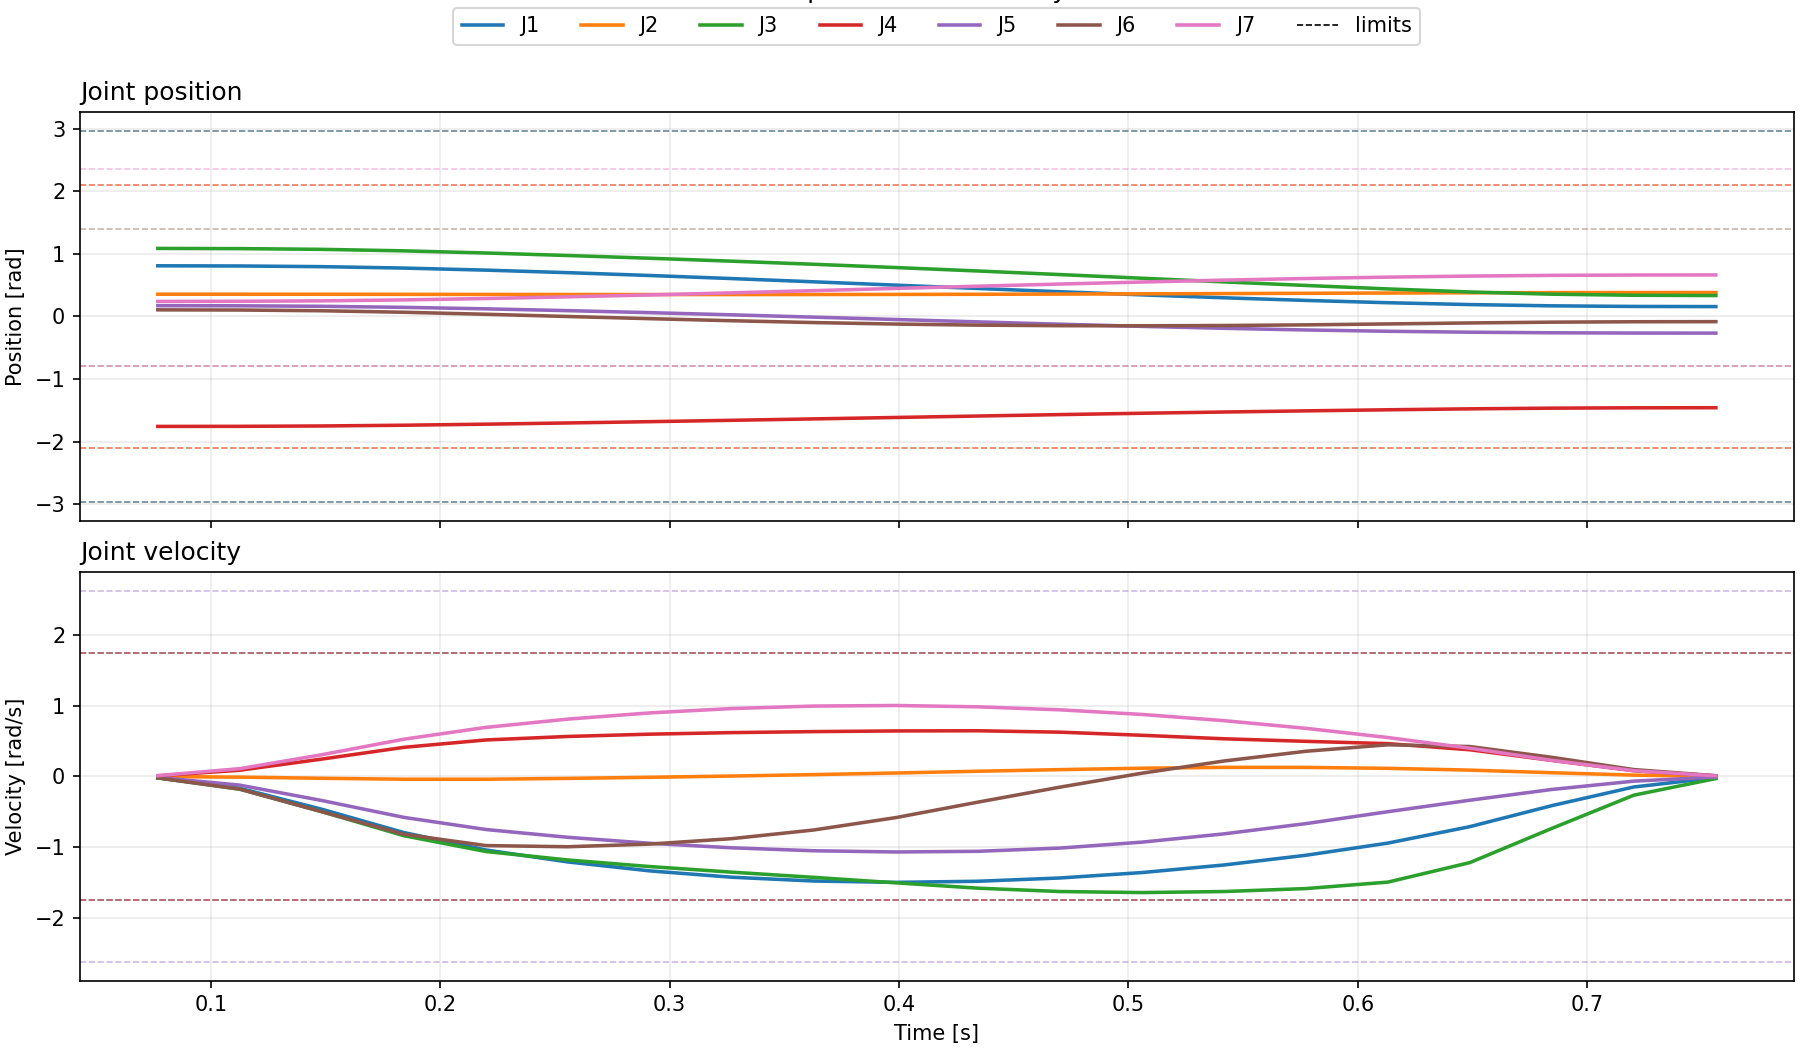
\includegraphics[width=\textwidth]{images/100GlobalRuns/row241_mc_example_position_velocity.png}
\caption{Joint positions and velocities for a representative MC solution of \ac{LUT} row 241. Dashed lines indicate the corresponding state limits.}
\label{fig:row241-mc-position-velocity}
\end{figure}

\begin{figure}[htbp]
\centering
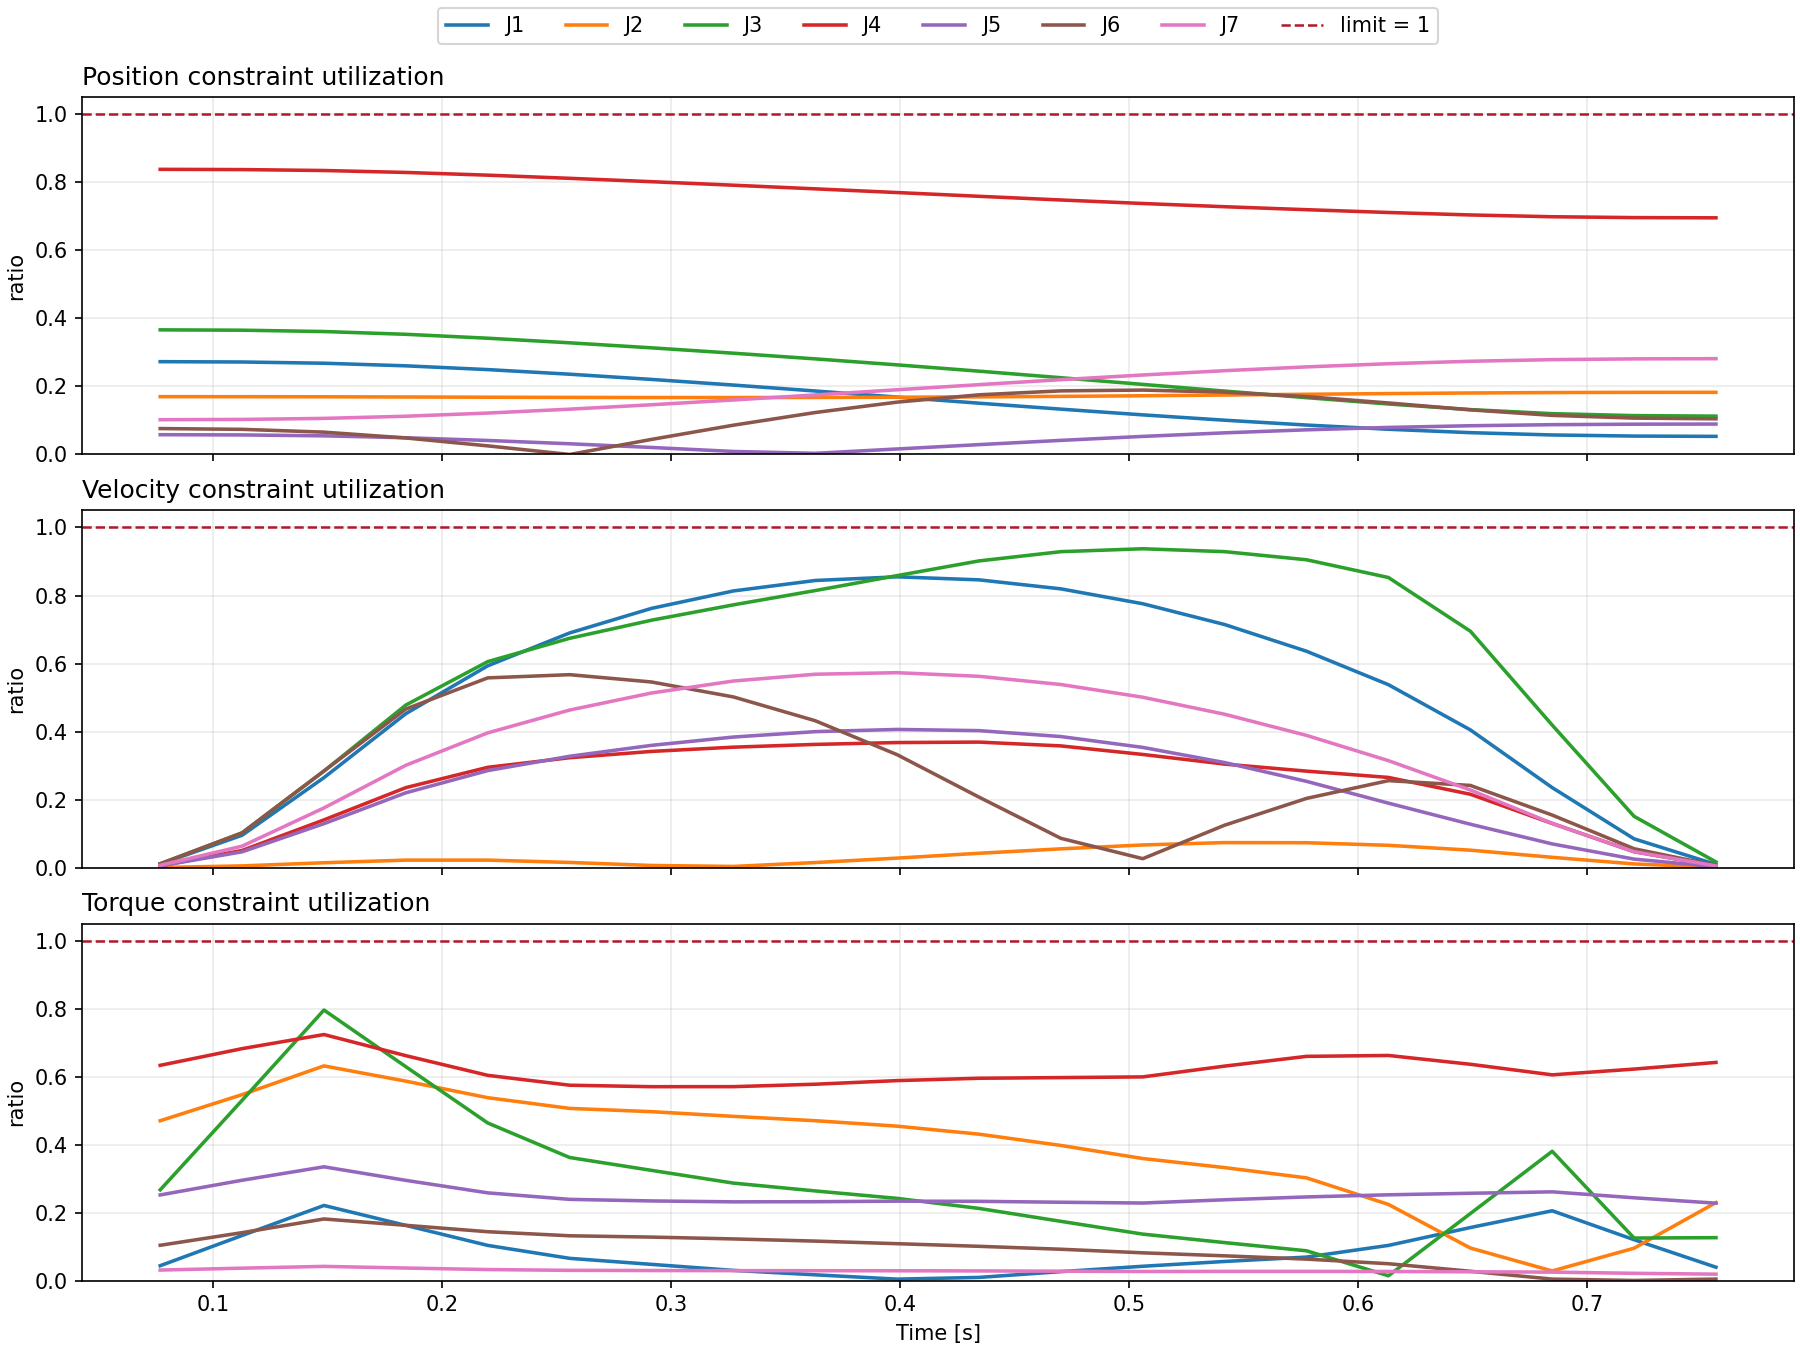
\includegraphics[width=\textwidth]{images/100GlobalRuns/row241_mc_example_ratios.png}
\caption{Normalized position, velocity, and torque constraint utilization for a representative MC solution of \ac{LUT} row 241. The red dashed line marks the unit utilization limit.}
\label{fig:row241-mc-constraint-utilization}
\end{figure}

\subsection{Robotic Manipulator Results Discussion}
\label{sec:results_manipulator_discussion}

\todoX{Summarize the main manipulator findings and relate them to the additional dynamic and terminal constraints.}
\todoX{Identify which methods best balance reliability, computation time, objective quality, and catch-trajectory diversity.}

\section{Cross-Model Algorithm Comparison}
\label{sec:results_cross_model}

\todoX{Provide a compact comparison of algorithm rankings across reliability, solution quality, computation time, and solution diversity for both models.}
\todoX{Explain which conclusions generalize across models and which are specific to spacecraft attitude or manipulator ball catching.}
\todoX{Discuss limitations caused by different workstation configurations, sample counts, time limits, or test-case difficulty.}

\section{Chapter Summary}
\label{sec:results_summary}

\todoX{Summarize the most important quantitative findings without introducing new analysis. Use this section to transition to the conclusions in \cref{ch:conclusion}.}
